\documentclass[12pt]{report}

\usepackage[utf8]{inputenc}
\usepackage{amssymb}
\usepackage{amsmath}
\usepackage{svg}
\usepackage{tabularx}
\usepackage{soul}
\usepackage[pdfusetitle]{hyperref}

\usepackage{geometry}
\geometry{
a4paper,
left=30mm,
right=30mm,
top=40mm,
bottom=30mm
}

\setcounter{secnumdepth}{3}

\usepackage{tikz}
\usetikzlibrary{circuits}
\usetikzlibrary{shapes,arrows}
\usetikzlibrary{positioning}

\tikzset{auto,>=latex', minimum size=0pt, node distance=1cm, font=\fontsize{11}{11}\selectfont}

\tikzstyle{block} = [draw, fill=white, rectangle, minimum height=3em, minimum width=4em, text centered, align=center]
\tikzstyle{integrator} = [draw, fill=white, rectangle, minimum height=3em, minimum width=2em, font={$\frac{1}{s}$}]
\tikzstyle{sum} = [draw, fill=white, circle, node distance=1cm]
\tikzstyle{input} = [coordinate]
\tikzstyle{output} = [coordinate]
\tikzstyle{pinstyle} = [pin edge={to-,thin,black}]
\tikzstyle{gain} = [draw, isosceles triangle, minimum height = 3em, isosceles triangle apex angle=60]
\tikzstyle{spy} = [coordinate, inner sep=0, outer sep=0, minimum size=0]
\tikzstyle{node} = [draw, circle, fill, minimum size=2pt, inner sep=0pt, outer sep=0pt, anchor=center]

%\usepackage{bodegraph}

%\usetikzlibrary{intersections}
%\usetikzlibrary{calc}

\setlength{\parindent}{0em}
\setlength{\parskip}{0.5em}

\newenvironment{conditions}
{\par\vspace{\abovedisplayskip}\noindent\centering\begin{tabular}{>{$}r<{$} @{${}:{}$} l}}
{\end{tabular}\par\vspace{\belowdisplayskip}}

\newenvironment{nb}{\par\vspace{\abovedisplayskip}\noindent\begin{em}n.b.\ \ignorespaces}{\end{em}}


\DeclareMathOperator{\im}{im}
\DeclareMathOperator{\rad}{rad}
\DeclareMathOperator{\sgn}{sgn}
\DeclareMathOperator{\diag}{diag}

\newcommand{\matr}[1]{\boldsymbol{#1}}
\newcommand{\vect}[1]{\boldsymbol{#1}}

\newcommand{\trans}{\mathsf{T}}
\newcommand{\inv}{{-1}}
\newcommand{\psinv}{\dag}
\newcommand\norm[1]{\left\lVert#1\right\rVert}

\newcommand{\Real}{\mathbb{R}}

\newcommand{\I}{\matr{I}}
\newcommand{\0}{\vect{0}}

\newcommand{\J}{\matr{J}}

\newcommand{\estimate}[1]{\hat{#1}}
\newcommand{\error}[1]{\tilde{#1}}
\newcommand{\reference}[1]{\bar{#1}}

\newcommand{\B}{\matr{B}}
\newcommand{\dB}{\dot\B}
\newcommand{\Bs}{\hat\B}
\newcommand{\Be}{\error\B}

\newcommand{\C}{\matr{C}}
\newcommand{\Cs}{\estimate\C}
\newcommand{\Ce}{\error\C}

\newcommand{\g}{\vect{g}}
\newcommand{\gs}{\estimate\g}

\newcommand{\n}{\vect{n}}
\newcommand{\ns}{\estimate\n}
\newcommand{\ner}{\error\n} % #r becuase ne already exists

\newcommand{\K}{\matr{K}}

\newcommand{\y}{\vect{y}}
\newcommand{\dy}{\dot{\y}}
\newcommand{\ddy}{\ddot{\y}}

\newcommand{\q}{\vect{q}}
\newcommand{\dq}{\dot{\q}}
\newcommand{\ddq}{\ddot{\q}}
\newcommand{\qd}{\bar{\q}}
\newcommand{\dqd}{\dot{\reference{\q}}}
\newcommand{\ddqd}{\ddot{\reference{\q}}}
\newcommand{\qe}{\error{\q}}
\newcommand{\dqe}{\dot{\error{\q}}}
\newcommand{\ddqe}{\ddot{\error{\q}}}
\newcommand{\qs}{\estimate{\q}}
\newcommand{\dqs}{\dot{\estimate{\q}}}
\newcommand{\ddqs}{\ddot{\estimate{\q}}}

\newcommand{\x}{\vect{x}}
\newcommand{\dx}{\dot{\x}}
\newcommand{\ddx}{\ddot{\x}}
\newcommand{\xd}{\reference{\x}}
\newcommand{\dxd}{\dot{\reference{\x}}}
\newcommand{\ddxd}{\ddot{\reference{\x}}}
\newcommand{\xe}{\error{\x}}
\newcommand{\dxe}{\dot{\error{\x}}}
\newcommand{\ddxe}{\ddot{\error{\x}}}
\newcommand{\xs}{\estimate{\x}}
\newcommand{\dxs}{\dot{\estimate{\x}}}
\newcommand{\ddxs}{\ddot{\estimate{\x}}}

\newcommand{\warning}[1]{\textcolor{red}{WARNING #1}}

\usepackage{imakeidx}
\makeindex[intoc]

\usepackage[backend=biber]{biblatex}
\addbibresource{references.bib}

\title{Control of industrial robots\\Notes\thanks{the whole document is based on \cite{cir-slides} and \cite{ssvo-robotics}}}
\author{Roberto Bochet}

\begin{document}

\maketitle

\printbibliography

\tableofcontents

\chapter{Kinematic redundancy}\label{ch:kinematic-redundancy}

We let $\vect{p}=k(\q)$ where $p$ is the pose of the end effector in the task space, $\q$ the joint configuration.
The kinematic function $k(\cdot)$ provides the transformation from the joint space $\mathbb{R}^n$ to the task space $\mathbb{R}^m$.

A robot is kinematically redundant if $n > m$.

\begin{nb}task space might be a subset of the operational space, so the dimension of the second one might be less than the first, that is why the redundancy is a relative concept\end{nb}

\section{Inverse kinematics}

\[ \q=k^{-1}(\vect{p}) \]

When a robot is kinematically redundant the inversion of the kinematics gives infinite solutions and there are internal motion that not affect the pose of the end effector.

To solve this issue the problem is usually addressed in the speed domain.

\begin{equation}
	\dot{\vect{p}} = \J(\q) \dq
	\label{eq:inverse-constraint}
\end{equation}

Where $\J(\q)$ is the Jacobian of the robot associated to the task space.

\subsection{Jacobian}

For a redundant robot the Jacobian are a rectangular matrix with the shape of $(m \times n)$ where $n > m$ as we saw before.

\[ \dim(\im(\J)) = m \quad \dim(\ker(\J)) = n - m \]

The null space exists only for a redundant robot.

So we can compose a movement as

\[ \dq = \dq^* + \matr{P} \dq_0 \quad \text{where} \quad \im(\matr{P}) \equiv \ker(\matr{J}) \]

with $P \dot{q}_0$ that does not contribute to the movement of the end effector, in fact if we multiply the equation to J from left we get

\[ \J\dq = \J\dq^* + \J P \dq_0 = \J \dq^* = \dot{\vect{p}} \]

where $J P \dq_0 = 0$ for each $\dq_0$.

\subsection{Finding a generic solution}

We can approach to the problem like a optimization one, as first thing we define a cost function in the joint space

\[ g(\dq) = \frac{1}{2} \dq^T \matr{W} \dq \]

$\matr{W}$ is a symmetrical weight matrix $(n \times n)$ and $\matr{W} > 0$

we want to find the optimal solution under the constraint $\dot{p} = \matr{W}(q) \dot{q}$ so we can use the Lagrange multiplier

\[ \mathcal{L}(\dq, \vect{\lambda}) = \frac{1}{2} \dq^T \matr{W} \dq + \lambda^T (\dot{p} - \J \dq)\]

\[
	\left(\frac{\partial \mathcal{L}}{\partial \dq}\right)^\trans = 0 \quad
	\left(\frac{\partial \mathcal{L}}{\partial \vect{\lambda}}\right)^\trans = 0
\]

from these we get

\[ \matr{W}\dq - \J^T\vect{\lambda} = 0 \qquad \dot{\vect{p}} - \J\dq = 0 \]

to combine the two equation we can find $\vect{\lambda}$

\[
\dot{\vect{p}} = \J\matr{W}^{-1}\J^\trans \vect{\lambda} \implies
\vect{\lambda} = (\J\matr{W}^{-1}\J^\trans)^{-1} \dot{\vect{p}}
\]

and with a recombination with the first equation we get the solution

\begin{gather*}
	\dq = \matr{W}^{-1} \J^\trans (\J\matr{W}^{-1}\J^\trans)^{-1} \dot{\vect{p}} \\
	\text{special case} \quad \matr{W} = \matr{I} \implies \dq = \J^\psinv \dot{\vect{p}}
\end{gather*}

The matrix $\J^\psinv = \J^\trans (\J\J^\trans)^{-1}$ is called \textbf{right pseudo inverse} matrix.
With dualism, we can define the matrix $\J^\psinv_W = \matr{W}^{-1} \J^\trans (\J\matr{W}^{-1}\J^\trans)^{-1}$ calling \textbf{weighted pseudo inverse} matrix.

\subsection{Finding a solution exploiting redundant}

As we saw before if $\dq^*$ is a valid solution to inverse problem also $\dq^* + \matr{P}\dq_0$ is it.
So, we can modify the general approach saw above to find a solution that exploiting the redundant.
We consider a new cost function

\[ g'(\dq) = \frac{1}{2} (\dq - \dq_0)^T (\dq - \dq_0) \]

To find a solution under the constraint \ref{eq:inverse-constraint} close to $\dq_0$.

\[ \mathcal{L}'(\dq, \vect{\lambda}) = \frac{1}{2} (\dq - \dq_0)^T (\dq - \dq_0) + \vect{\lambda}^T (\dot{\vect{p}} - \J \dq) \]

From $\frac{\partial \mathcal{L}'}{\partial \dq} = 0$ and the constraint~\ref{eq:inverse-constraint} we can get $\vect{\lambda}$

\[\vect{\lambda} = (\J\J^\trans)^{-1} (\dot{\vect{p}} - \J\dq_0)\]

then we get the solution

\[ \dq = \J^\psinv \dot{\vect{p}} + (\matr{I} - \J^\psinv \J) \dq_0 \]

So we found $(\matr{I} - \J^\psinv \J)$ a solution for the matrix $\matr{P}$.

\subsubsection{Choosing $\dq_0$}

Now we can choose $\dq_0$ to improve the behaviour of the robot exploiting its redundancy.
A typical choice of $\dq_0$ called \textbf{projected gradient} has the shape

\[ \dq_0 = k_0 \left(\frac{\partial w(\q)}{\partial \q}\right)^\trans \]

Choosing $w(\q)$ as a cost function to maximize to increase a specific performance:

\begin{itemize}
	\item \textbf{Manipulability} measure to maximize the distance from singularities
	\[ w(\q) = \sqrt{\det(\J(\q)\J^\trans(\q))} \]

	\item Distance form \textbf{joint limits}
	\[ w(\q) = \frac{1}{2n} \sum_{i=1}^{n} \left( \frac{q_i - \bar{q}_i}{q_{iM} - \bar{q}_{im}} \right)^2 \]

	\item Distance from the \textbf{closet obstacle}
	\[ w(\q) = \min_{\vect{p},\vect{o}}\norm{\vect{p}(\q)-\vect{o}} \]
\end{itemize}

$k_0 > 0$ can be arbitrary chosen. 

\subsection{Possible issues with redundant robots}

Mainly two possible issues

\begin{itemize}
	\item A close trajectory in the task space can be mapped as a open trajectory in the joint space
	\item Trajectories with the same initial and final task positions may end with different joint configurations
\end{itemize}

A possible solution to these problems is the method called \textbf{repeatable} or \textbf{cyclic}


\warning{missing ciclicity, extended jacobian, and control}


\chapter{Robot dynamics}
\chapter{Motion planning}
\chapter{Decentralized control}\label{ch:decentralized-control}

Once a desired robot trajectory is designed, the next step is to guarantee that the real trajectory as close as possible to it.
Practically we have to design a control strategy in order to $\q_d(t) \approx \q(t)$.

The main way adopted in the control of industrial robot is the \textbf{independent joint control}\index{independent joint control} approach;
it is a decentralized control approach where each joint is controlled independently of each other.

\warning{Missing evaluation of control performance}

\section{Simplified dynamic model}\label{sec:simplified-dynamic-model}

Let us consider a simplified dynamics model of the robots

\[
    \matr{B}(\q)\ddq + \matr{C}(\q,\dq)\dq + \vect{g}(\q) = \vect{\tau}
\]

In this model $\vect{\tau}, \q, \dq, \ddq$ are referred to the joints, but in a real system we cannot act directly on the joints variables, instead we have to consider that we can act only on the motors that are bound to the joints via a transmission.
So we introduce a dynamics model for a generic rigid transmission and joint motor

\begin{gather*}
    J_{mi}\ddot{q}_{m_i} + D_{m_i}\dot{q}_{m_i} = \tau_{m_i} - \tau_{lm_i} \\
    \tau_{lm_i} = \tau_{l_i} / n_i
\end{gather*}
where
\begin{conditions}
    J_{m_i} & moment of inertial of the motor \\
    D_{m_i} & friction viscous coefficient of the motor \\
    \tau_{lm_i} & load torque on the axis of the motor \\
    \tau_{l_i} & load torque on the axis of the joint \\
    n_i & transmission reduction rate between motor and joint
\end{conditions}

to simplify we considered just the effect related to its spinning around its own axis and a rigid transmission.

Let us introduce the square matrix $\matr N = \diag\{n_i\}$ so we can write

\[
    \q_m = \matr N \q \qquad \vect \tau_{lm} = \matr N^{-1} \vect \tau
\]

Before we consider the entire model seen from the motor point of view, we observe that the matrix $\matr B(\q)$ can be seen as the sum of two contributes, the first of average inertia and the other of the residual as function of the pose $\q$

\[
    \matr B(\q) = \bar{\matr B} + \matr{\Delta B}(\q)
\]

Now we can combine the models of motors/transmissions and robots

\begin{align*}
    \matr J_m\ddq_m + \matr D_m \dq_m &= \vect \tau_m - \vect \tau_{lm} \\
    \matr J_m\ddq_m + \matr D_m \dq_m + \matr N^{-1} \left( \matr{B}(\q)\ddq +
    \matr{C}(\q,\dq)\dq + \vect{g}(\q) \right) &= \vect \tau_m \\
    \intertext{replace the joints variables with motors ones} \\
    \matr J_m\ddq_m + \matr D_m \dq_m + \matr N^{-1} \matr{B}(\q) \matr N^{-1} \ddq_m +
    \matr N^{-1} \matr{C}(\q,\dq) \matr N^{-1} \dq_m +
    \matr N^{-1} \vect{g}(\q) &= \vect \tau_m \\
    \intertext{introduce the decomposition of $\matr B(\q)$} \\
    \matr J_m\ddq_m + \matr D_m \dq_m + \matr N^{-1} \left(\bar{\matr B} + \matr{\Delta B}(\q)\right) \matr N^{-1} \ddq_m +
    \matr N^{-1} \matr{C}(\q,\dq) \matr N^{-1} \dq_m +
    \matr N^{-1} \vect{g}(\q) &= \vect \tau_m \\
    (\matr J_m + \matr N^{-1} \bar{\matr B} \matr N^{-1} )\ddq_m + \matr D_m \dq_m + \hspace{7cm} \\
    \matr N^{-1} \matr{\Delta B}(\q) \matr N^{-1} \ddq_m +
    \matr N^{-1} \matr{C}(\q,\dq) \matr N^{-1} \dq_m +
    \matr N^{-1} \vect{g}(\q) &= \vect \tau_m \\
    \intertext{introduce the vector $\vect d$ and the matrix $\bar{\matr B}_r = \matr N^{-1} \bar{\matr B} \matr N^{-1}$} \\
    \left(\matr J_m + \bar{\matr B}_r \right)\ddq_m + \matr D_m \dq_m + \vect d &= \vect \tau_m
\end{align*}

where

\begin{equation}
    \vect d = \matr N^{-1} \matr{\Delta B}(\q) \matr N^{-1} \ddq_m +\matr N^{-1} \matr{C}(\q,\dq) \matr N^{-1} \dq_m + \matr N^{-1} \vect{g}(\q)\label{eq:decentralized-noise}
\end{equation}

We got a dynamics model where the motor torques $\vect \tau_m$ are the input, and the vector $\vect d$ is a non-linear function that we can treat as noise, you can see it in the \autoref{fig:mtj-model}.

\begin{nb}all the non-linearities are moved in the noise $\vect d$.\end{nb}
\begin{nb}the bigger are the reduction ratios $n_i$, the less relevant the noise $\vect d$ is.\end{nb}

So, the decentralized control approach treat each joint as a SISO linear model subject to a noise.
The control loop for each joint is independent of each others.

\ul{This method heavily relies on the assumption that the reduction ratios $n_i$ values are large} (generally true for industrial robotics manipulators), \ul{to can ignore the nonlinear contribution $\vect d$ in the controller design.}

\begin{figure}[htb]
    \centering
    %\resizebox{\textwidth}{!}{
    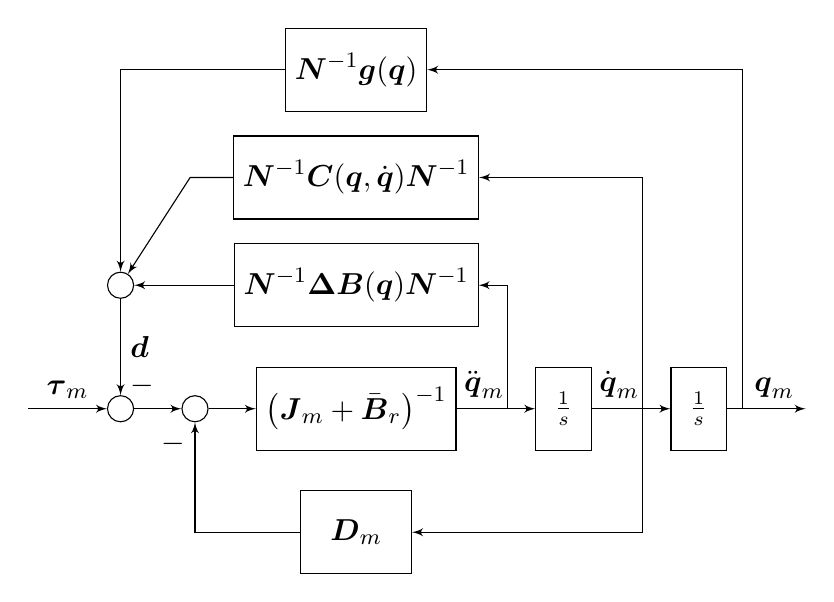
\begin{tikzpicture}
        \node [input] (input) {};
        \node [sum, right=1cm of input] (sum_i) {};
        \node [sum, right=0.6cm of sum_i] (sum_f) {};
        \node [block, right=0.6cm of sum_f] (inertial) {$\left(\matr J_m + \bar{\matr B}_r \right)^{-1}$};
        \node [block, below=0.5cm of inertial] (dq2f) {$\matr D_m$};
        \node [integrator, right=1cm of inertial] (ddq2dq) {};
        \node [integrator, right=1cm of ddq2dq] (dq2q) {};
        \node [output, right=1cm of dq2q] (output) {};
        \node [block, above=0.5cm of inertial] (d_b) {$\matr N^{-1} \matr{\Delta B}(\q) \matr N^{-1}$};
        \node [block, above=0.3cm of d_b] (d_c) {$\matr N^{-1} \matr{C}(\q,\dq) \matr N^{-1}$};
        \node [block, above=0.3cm of d_c] (d_g) {$\matr N^{-1} \vect{g}(\q)$};
        \node [sum] (sum_d) at (sum_i |- d_b)  {};

        \draw [->] (input) -- node {$\vect \tau_m$} (sum_i);
        \draw [->] (sum_i) -- (sum_f);
        \draw [->] (sum_f) -- (inertial);
        \draw [->] (sum_d) -- node [pos=0.9] {$-$} node [pos=0.5] {$\vect d$} (sum_i);
        \draw [->] (d_b) -- (sum_d);
        \draw [->] (d_c) -- ++(-6em,0) -- (sum_d);
        \draw [->] (d_g) -| (sum_d);
        \draw [->] (inertial) -- node [pos=0.35] {$\ddq_m$} node [name=ddq, pos=0.65,inner sep=0] {}  (ddq2dq);
        \draw [->] (ddq2dq) -- node [pos=0.35] {$\dq_m$} node [name=dq, pos=0.65,inner sep=0] {}  (dq2q);
        \draw [->] (dq2q) -- node [name=q, pos=0.2,inner sep=0] {} node [pos=0.6] {$\q_m$}  (output);

        \draw [->] (ddq) |- (d_b);
        \draw [->] (dq) |- (d_c);
        \draw [->] (q) |- (d_g);

        \draw [->] (dq) |- (dq2f);
        \draw [->] (dq2f) -| node [pos=0.9] {$-$} (sum_f);
    \end{tikzpicture}
    %}
    \caption{motor-transmission-joint dynamics model \\ \begin{em}n.b.\ the arrows for the dependencies of noise functions are been omitted\end{em}}
    \label{fig:mtj-model}
\end{figure}

\section{Electrical motor}

Let's consider a simple DC motor

\begin{align*}
    V(t) &= R i(t) + L \dot{i}(t) + E(t) \\
    E(t) &= K \dot{q}_m(t) \\
    \tau_m(t) &= K i(t) = J_m \ddot{q}_m(t)
\end{align*}

\begin{figure}[htb]
\centering
\resizebox{\textwidth}{!}{
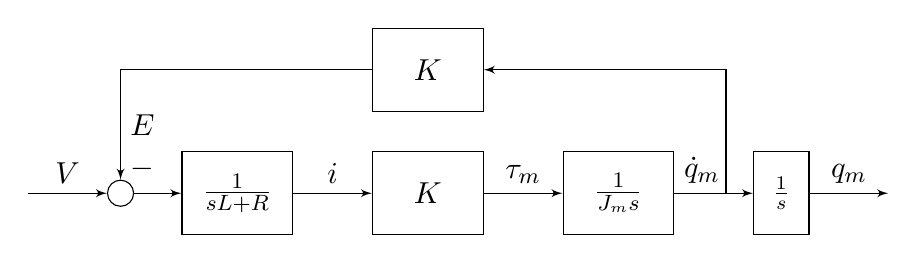
\begin{tikzpicture}
    \node [input] (input) {};
    \node [sum, right= 1cm of input] (sum_v) {};
    \node [block, right=0.6cm of sum_v] (v2i) {$\frac{1}{sL+R}$};
    \node [block, right=1cm of v2i] (i2tau) {$K$};
    \node [block, above=0.5cm of i2tau] (dq2e) {$K$};
    \node [block, right=1cm of i2tau] (tau2dq) {$\frac{1}{J_m s}$};
    \node [integrator, right=1cm of tau2dq] (dq2q) {};
    \node [output, right=1cm of dq2q] (output) {};
    
    \draw [draw,->] (input) -- node {$V$} (sum_v);
    \draw [->] (sum_v) -- (v2i);
    \draw [->] (v2i) -- node {$i$} (i2tau);
    \draw [->] (i2tau) -- node {$\tau_m$} (tau2dq);
    \draw [->] (tau2dq) -- node [pos=0.35] {$\dot{q}_m$} node [name=dq, pos=0.65,inner sep=0] {}  (dq2q);
    \draw [->] (dq2q) -- node {$q_m$} (output);
    \draw [->] (dq.0) |- (dq2e);
    \draw [->] (dq2e) -| node [pos=0.95] {$-$} node [near end] {$E$} (sum_v);
\end{tikzpicture}
}
\caption{DC motor model}
\label{fig:motor_model}
\end{figure}

\subsection{Control of the current}

We can close a high frequency (thousands $\rad/s$) loop for the current as it can be seen in \autoref{fig:motor_current_control}. $E$ is considered to change as a slowly varying disturbance, that the controller can effectively reject.
From the point of view of the mechanical system the current loop is so fast to consider the current change is instantaneous.
So for the mechanical control we can consider to control directly the motor torque

\[
    \tau_m(t) = Ki(t) \approx K \bar{i}(t)
\]

\begin{figure}[htb]
\centering
\resizebox{\textwidth}{!}{
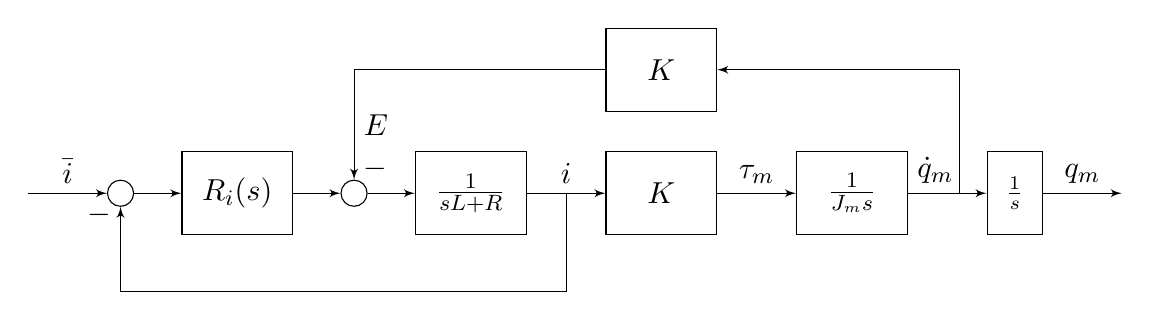
\begin{tikzpicture}
    \node [input] (input) {};
    \node [sum, right= 1cm of input] (sum_e) {};
    \node [block, right=0.6cm of sum_e] (e2v) {$R_i(s)$};
    \node [sum, right= 0.6cm of e2v] (sum_v) {};
    \node [block, right=0.6cm of sum_v] (v2i) {$\frac{1}{sL+R}$};
    \node [block, right=1cm of v2i] (i2tau) {$K$};
    \node [block, above=0.5cm of i2tau] (dq2e) {$K$};
    \node [block, right=1cm of i2tau] (tau2dq) {$\frac{1}{J_m s}$};
    \node [integrator, right=1cm of tau2dq] (dq2q) {};
    \node [output, right=1cm of dq2q] (output) {};
    
    \draw [draw,->] (input) -- node {$\bar{i}$} (sum_e);
    \draw [->] (sum_e) -- (e2v);
    \draw [->] (e2v) -- (sum_v);
    \draw [->] (sum_v) -- (v2i);
    \draw [->] (v2i) -- node [name=i] {$i$} (i2tau);
    \draw [->] (i) -- ++ (0,-1.5) -| node [pos=0.95] {$-$} (sum_e);
    \draw [->] (i2tau) -- node {$\tau_m$} (tau2dq);
    \draw [->] (tau2dq) -- node [pos=0.35] {$\dot{q}_m$} node [name=dq, pos=0.65,inner sep=0] {}  (dq2q);
    \draw [->] (dq2q) -- node {$q_m$} (output);
    \draw [->] (dq.0) |- (dq2e);
    \draw [->] (dq2e) -| node [pos=0.95] {$-$} node [near end] {$E$} (sum_v);
\end{tikzpicture}
}
\caption{motor current control}
\label{fig:motor_current_control}
\end{figure}

\section{Rigid transmission approximation}

As we saw above, for a rigid transmission we have the following system

\begin{gather*}
    J_m\ddot{q}_m + d_m \dot{q}_m = \tau_m - \tau_{lm}\\
    J_l\ddot{q}_l = n \tau_{lm} - \tau_l\\
    q_m = n q_l\\
\end{gather*}

The first and the second equation can be merged exploiting the third equation

\[
    \left(J_m + \frac{J_l}{n^2}\right) \ddot{q}_m + d_m \dot{q}_m = \tau_m - \frac{\tau_l}{n}
\]

The result model can be seen in the \autoref{fig:mechanical_system_rigid}

\[
    G_v(s) = \frac{1}{d_m + \left(J_m + \frac{J_l}{n^2}\right) s} = \frac{1/d_m}{1 + \frac{J_m + J_l/n^2}{d_m} s}
\]

$d_m$ is an uncertain small parameter, since $d_m$ give a real stable pole we can consider the most conservative situation in which $d_m=0$, so we get

\[
    G_v(s) = \frac{1}{\left(J_m + \frac{J_l}{n^2}\right) s}
\]

\begin{figure}[htb]
\centering
\resizebox{0.6\textwidth}{!}{%
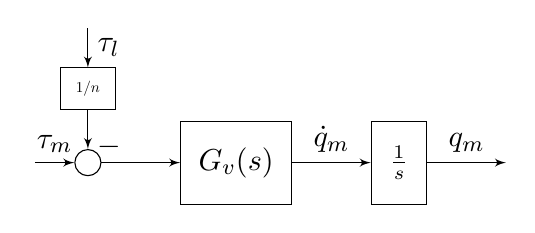
\begin{tikzpicture}
    \node [input, name=tau_m] {};
    \node [sum, right= 0.5cm of tau_m] (sum_tau) {};
    \node [block, above=0.5cm of sum_tau, scale=0.5] (taul2taulr) {$1/n$};
    \node [input, above=0.5cm of taul2taulr, name=tau_l] {};
    \node [block, right=1cm of sum_tau] (tau2dqm) {$G_v(s)$};
    \node [integrator, right=1cm of tau2dqm] (dqm2qm) {};
    \node [output, right=1cm of dqm2qm] (q_m) {};
    
    \draw [->] (tau_m) -- node {$\tau_m$} (sum_tau);
    \draw [->] (tau_l) -- node {$\tau_l$} (taul2taulr);
    \draw [->] (taul2taulr) -- node [pos=0.95] {$-$} (sum_tau);
    \draw [->] (sum_tau) -- (tau2dqm);
    \draw [->] (tau2dqm) -- node {$\dot{q}_m$} (dqm2qm);
    \draw [->] (dqm2qm) -- node {$q_m$} (q_m);
\end{tikzpicture}
}%
\caption{Mechanical system with rigid transmission}
\label{fig:mechanical_system_rigid}
\end{figure}

\subsection{P/PI control}

In order to control position of the motor we can close in cascade two loop (also to the current loop).
The first with a \textbf{PI} regulator on the motor speed and the second with an \textbf{P} regulator on the motor position as you can see in \autoref{fig:rigid_control_position}.

\begin{nb}in \autoref{fig:rigid_control_position} the current loop is omitted because, as we said before, the current loop has a much higher bandwidth than the speed loop, so we can assume $\bar{\tau}_m=\tau_m$.\end{nb}

\begin{figure}[htb]
\centering
\resizebox{\textwidth}{!}{
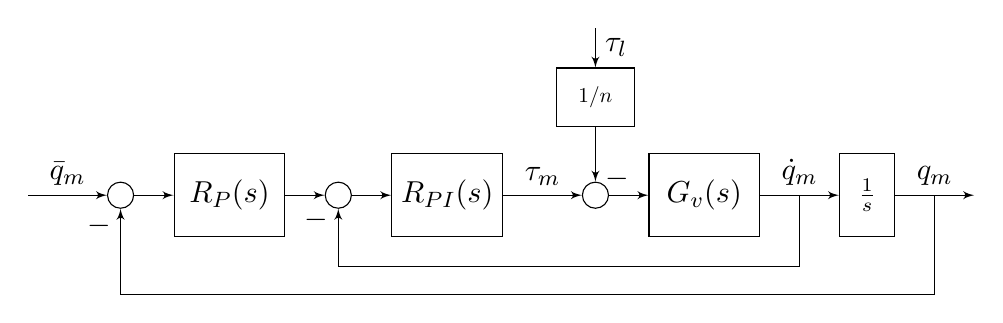
\begin{tikzpicture}
    \node [input] (input) {};
    \node [sum, right=1cm of input] (sum_p) {};
    \node [block, right=.5cm of sum_p] (p) {$R_{P}(s)$};
    \node [sum, right=.5cm of p] (sum_v) {};
    \node [block, right=.5cm of sum_v] (pi) {$R_{PI}(s)$};
    \node [sum, right=1cm of pi] (sum_tau) {};
    \node [block, above=.7cm of sum_tau, scale=.7] (taul2taulr) {$1/n$};
    \node [input, above=.5cm of taul2taulr, name=tau_l] {};
    \node [block, right=.5cm of sum_tau] (tau2dqm) {$G_{v}(s)$};
    \node [integrator, right=1cm of tau2dqm] (dqm2qm) {};
    \node [output, right=1cm of dqm2qm] (output) {};
    
    \draw [draw,->] (input) -- node {$\bar{q}_m$} (sum_p);
    \draw [->] (sum_p) -- (p);
    \draw [->] (p) -- (sum_v);
    \draw [->] (sum_v) -- (pi);
    \draw [->] (pi) -- node {$\tau_m$} (sum_tau);
    \draw [->] (tau_l) -- node {$\tau_l$} (taul2taulr);
    \draw [->] (taul2taulr) -- node [pos=0.95] {$-$} (sum_tau);
    \draw [->] (sum_tau) -- (tau2dqm);
    \draw [->] (tau2dqm) -- node [name=dq_m] {$\dot{q}_m$} (dqm2qm);
    \draw [->] (dqm2qm) -- node [name=q_m] {$q_m$} (output);
    \draw [->] (dq_m) -- ++ (0,-1.2) -| node [pos=0.9] {$-$} (sum_v);
    \draw [->] (q_m) -- ++ (0,-1.5) -| node [pos=0.9] {$-$} (sum_p);
\end{tikzpicture}
}
\caption{Control scheme P/PI with a rigid transmission}
\label{fig:rigid_control_position}
\end{figure}

\subsubsection{PI speed control design}

As we stated the P/PI design is done with cascade approach, so as first step we can design the speed loop.

\[
    R_{PI}(s) = k_{pv} \frac{1 + t_{iv} s}{s} \implies
    L_v(s) = \frac{k_{pv}}{\left(J_m + \frac{J_l}{n^2}\right)} \frac{1 + t_{iv} s}{s^2}
\]

We impose an $\omega_{cv}$ with $k_{pv}$

\[ \omega_{cv}=\frac{k_{pv}}{\left(J_m + \frac{J_l}{n^2}\right)} \]

and to guarantee that the $\omega_{cv}$ desired coincide with the effective one we have to put the zero in low frequency respect it

\[ t_{iv} \approx \frac{1}{(0.1 \div 0.3)\omega_{cv}} \]

With this regulator we get a close loop function for the speed loop 

\[ F_v(s) \approx \frac{1}{1 + \frac{1}{\omega_{cv}}s} \]

\subsubsection{P position control design}

We can now design the $R_P(s)$ controller taking in account the speed closed loop designed above.

\[
R_{P}(s) = k_{pp} \implies
L_p(s) = k_{pp} \frac{1}{s \left(1 + \frac{1}{\omega_{cv}} s\right)}
\]

if we choose $\omega_{cp} \ll \omega_{cv}$ is enough to impose $k_{pp} = \omega_{cp}$

The overall closed loop on the position guarantee null static error and a bandwidth of $\omega_{cp}$.

\subsubsection{Speed feed-forward}

A possible improvement of the \textbf{P/PI} scheme is the speed feed-forward scheme \autoref{fig:rigid_control_ff}.
The block $k_{ff}s$ improves the speed of the response of the position control.
The $k_{ff}$ coefficient is chosen between 0 and 1.

\begin{figure}[htb]
\centering
\resizebox{\textwidth}{!}{
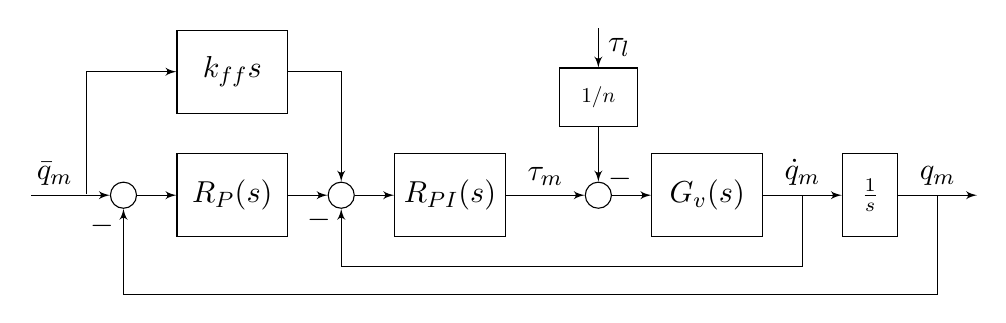
\begin{tikzpicture}
    \node [input] (input) {};
    \node [sum, right=1cm of input] (sum_p) {};
    \node [block, right=.5cm of sum_p] (r_p) {$R_{P}(s)$};
    \node [block, above=.5cm of r_p] (ff) {$k_{ff}s$};
    \node [sum, right=.5cm of r_p] (sum_v) {};
    \node [block, right=.5cm of sum_v] (r_v) {$R_{PI}(s)$};
    \node [sum, right=1cm of r_v] (sum_tau) {};
    \node [block, above=.7cm of sum_tau, scale=.7] (taul2taulr) {$1/n$};
    \node [input, above=.5cm of taul2taulr, name=tau_l] {};
    \node [block, right=.5cm of sum_tau] (tau2dqm) {$G_{v}(s)$};
    \node [integrator, right=1cm of tau2dqm] (dqm2qm) {};
    \node [output, right=1cm of dqm2qm] (output) {};
    
    \draw [draw,->] (input) -- node [pos=0.3] {$\bar{q}_m$} node [name=rqm, pos=0.7,inner sep=0] {} (sum_p);
    \draw [->] (sum_p) -- (r_p);
    \draw [->] (r_p) -- (sum_v);
    \draw [->] (rqm) |- (ff);
    \draw [->] (ff) -| (sum_v);
    \draw [->] (sum_v) -- (r_v);
    \draw [->] (r_v) -- node {$\tau_m$} (sum_tau);
    \draw [->] (tau_l) -- node {$\tau_l$} (taul2taulr);
    \draw [->] (taul2taulr) -- node [pos=0.95] {$-$} (sum_tau);
    \draw [->] (sum_tau) -- (tau2dqm);
    \draw [->] (tau2dqm) -- node [name=dq_m] {$\dot{q}_m$} (dqm2qm);
    \draw [->] (dqm2qm) -- node [name=q_m] {$q_m$} (output);
    \draw [->] (dq_m) -- ++ (0,-1.2) -| node [pos=0.9] {$-$} (sum_v);
    \draw [->] (q_m) -- ++ (0,-1.5) -| node [pos=0.9] {$-$} (sum_p);
\end{tikzpicture}
}
\caption{Control scheme P/PI with a rigid transmission and speed feed-forward}
\label{fig:rigid_control_ff}
\end{figure}

\subsubsection{Position measure only}

If only available the position measure but not the speed, it can be derived with a process of differentiation on the position. The control scheme became as \autoref{fig:rigid_control_position_only} that are equivalent to \autoref{fig:rigid_control_position_only_pid} where all the controller block are substituted with a single \textbf{PID} on position loop.


\begin{figure}
\centering
\resizebox{\textwidth}{!}{
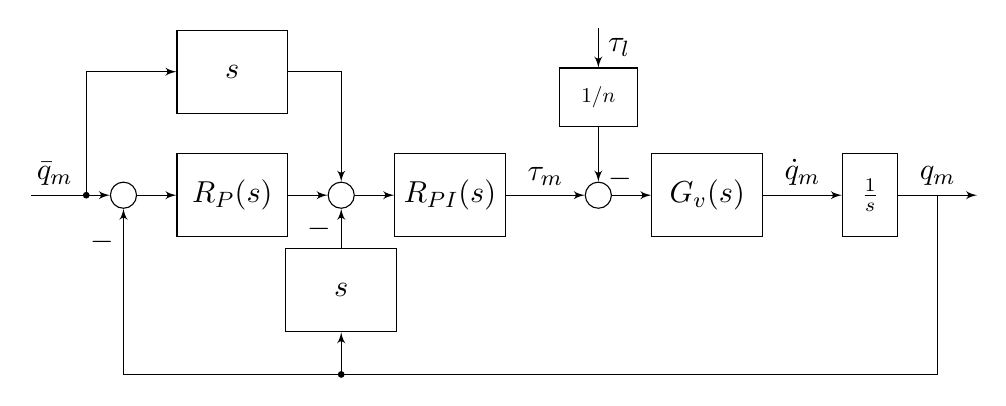
\begin{tikzpicture}
    \node [input] (input) {};
    \node [sum, right=1cm of input] (sum_p) {};
    \node [block, right=.5cm of sum_p] (r_p) {$R_{P}(s)$};
    \node [block, above=.5cm of r_p] (ff) {$s$};
    \node [sum, right=.5cm of r_p] (sum_v) {};
    \node [block, below=.5cm of sum_v] (d) {$s$};
    \node [node, below=.5cm of d] (fq_m) {};
    \node [block, right=.5cm of sum_v] (r_v) {$R_{PI}(s)$};
    \node [sum, right=1cm of r_v] (sum_tau) {};
    \node [block, above=.7cm of sum_tau, scale=.7] (taul2taulr) {$1/n$};
    \node [input, above=.5cm of taul2taulr, name=tau_l] {};
    \node [block, right=.5cm of sum_tau] (tau2dqm) {$G_{v}(s)$};
    \node [integrator, right=1cm of tau2dqm] (dqm2qm) {};
    \node [output, right=1cm of dqm2qm] (output) {};
    
    \draw [draw,->] (input) -- node [pos=0.3] {$\bar{q}_m$} node [node, name=rqm, pos=0.7] {} (sum_p);
    \draw [->] (sum_p) -- (r_p);
    \draw [->] (r_p) -- (sum_v);
    \draw [->] (rqm) |- (ff);
    \draw [->] (ff) -| (sum_v);
    \draw [->] (sum_v) -- (r_v);
    \draw [->] (r_v) -- node {$\tau_m$} (sum_tau);
    \draw [->] (tau_l) -- node {$\tau_l$} (taul2taulr);
    \draw [->] (taul2taulr) -- node [pos=0.95] {$-$} (sum_tau);
    \draw [->] (sum_tau) -- (tau2dqm);
    \draw [->] (tau2dqm) -- node [name=dq_m] {$\dot{q}_m$} (dqm2qm);
    \draw [->] (dqm2qm) -- node [name=q_m] {$q_m$} (output);
    \draw [->] (d) -- node [pos=0.5] {$-$} (sum_v);
    \draw [->] (fq_m) -- (d);
    \draw [->] (q_m) |- (fq_m) -| node [pos=0.9] {$-$} (sum_p);
\end{tikzpicture}
}
\caption{Control scheme with only position measurement}
\label{fig:rigid_control_position_only}
\end{figure}

\begin{figure}
\centering
\resizebox{\textwidth}{!}{
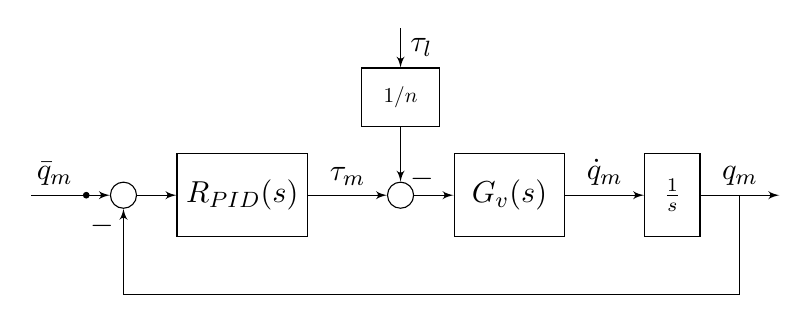
\begin{tikzpicture}
    \node [input] (input) {};
    \node [sum, right=1cm of input] (sum_p) {};
    \node [block, right=.5cm of sum_p] (r) {$R_{PID}(s)$};
    \node [sum, right=1cm of r] (sum_tau) {};
    \node [block, above=.7cm of sum_tau, scale=.7] (taul2taulr) {$1/n$};
    \node [input, above=.5cm of taul2taulr, name=tau_l] {};
    \node [block, right=.5cm of sum_tau] (tau2dqm) {$G_{v}(s)$};
    \node [integrator, right=1cm of tau2dqm] (dqm2qm) {};
    \node [output, right=1cm of dqm2qm] (output) {};
    
    \draw [draw,->] (input) -- node [pos=0.3] {$\bar{q}_m$} node [node, name=rqm, pos=0.7] {} (sum_p);
    \draw [->] (sum_p) -- (r);
    \draw [->] (r) -- node {$\tau_m$} (sum_tau);
    \draw [->] (tau_l) -- node {$\tau_l$} (taul2taulr);
    \draw [->] (taul2taulr) -- node [pos=0.95] {$-$} (sum_tau);
    \draw [->] (sum_tau) -- (tau2dqm);
    \draw [->] (tau2dqm) -- node [name=dq_m] {$\dot{q}_m$} (dqm2qm);
    \draw [->] (dqm2qm) -- node [name=q_m] {$q_m$} (output);
    \draw [->] (q_m) -- ++ (0, -1.5) -| node [pos=0.9] {$-$} (sum_p);
\end{tikzpicture}
}
\caption{Control scheme PID with only position measurement}
\label{fig:rigid_control_position_only_pid}
\end{figure}

\section{Elastic transmission}

If we look only to the rigid transmission model we do not find significant limitations in the bandwidth of speed control, but from experimental data we can clearly find several limitations mainly bound to vibration, we have to improve the rigid model to take in account these limitations.

If we consider an elastic transmission we can write the following system

\begin{gather*}
    J_m\ddot{q}_m + d_m \dot{q}_m = \tau_m - \tau_{lm}\\
    J_l\ddot{q}_l = n \tau_{lm} - \tau_l\\
    \tau_{lm} = k_{el}(q_m - n q_l) + d_{el}(\dot{q}_m - n \dot{q}_l)\\
\end{gather*}

The $G_v(s)$ now is composed of one real pole, two complex poles and two complex zeros;
in particular we can find the parameter $\omega_z$ of the complex zeros as

\[\omega_z = \sqrt{\frac{k_{el}}{J_l}}\]

and a reasonable choice for the speed closed loop bandwidth is $\omega_{cv} \approx 0.7 \omega_z$

\chapter{Centralized control}\label{ch:centralized-control}

As opposed of the decentralized approach where each joint is controlled independently of each others, we can implement a control law based on \textbf{centralized approach}\index{centralized control approach} where the manipulator is controlled exploiting its overall model.
This approach required obviously a model of the robot, but it generally guarantees better performance than the decentralized one.

\begin{nb}as we saw in \autoref{sec:simplified-dynamic-model} for a \textbf{decentralized} control we stated that a high reduction ratios in transmissions between motors and joints is a fundamental requirement because this reduces the magnitude of the noise $\vect d$, if this decoupling effect is not guaranteed we must use the \textbf{centralized} approach.\end{nb}

The \textbf{centralized control approach} allows us to develop several control schemes both in the joint space that in the operational one.

\section{Control in joint space}

In joint space control the design of the controller is done directly on the joints state.

\subsection{Open loop}

A first naive approach can be seen as an extension of a \textbf{decentralized controller} designed in the previous chapter.

The idea is to compensate the noise $\vect d$ adding to the decentralized scheme an open loop controller fed with the desired joints functions $\qd, \dqd, \ddqd$.
Yuo can see the scheme in \autoref{fig:open-loop}.

The function of the feedforward controller can be designed from \autoref{eq:decentralized-noise} using as input the desired state

\[
	\hat{\vect d} = \matr N^{-1} \matr{\Delta B}(\qd) \matr N^{-1} \ddqd_m +\matr N^{-1} \matr{C}(\qd,\dqd) \matr N^{-1} \dqd_m + \matr N^{-1} \vect{g}(\qd)
\]

The calculation of $\hat{\vect d}$ is generally computationally expensive, so it is preferred to precalculate it offline $\hat{\vect d}$ if it is possible (i.e in the repeated trajectories).

\begin{figure}[htb]
	\centering
	\resizebox{\textwidth}{!}{
	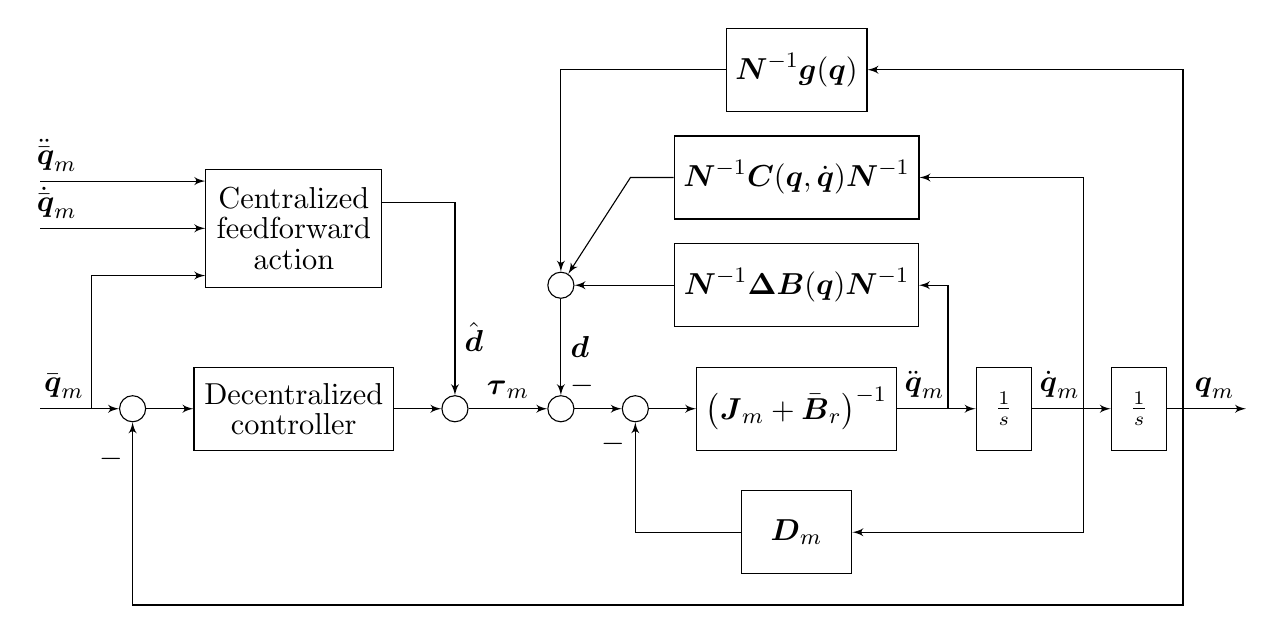
\begin{tikzpicture}
		\node [input] (iq_d) {};
		\node [sum, right= 1cm of iq_d] (sum_e) {};
		\node [block, right=0.6cm of sum_e, text width=2.3cm] (controller) {Decentralized\\controller};
		\node [block, above=1cm of controller, text width=2cm, minimum height=1.5cm] (controller_ff) {Centralized feedforward action};
		\node [sum, right=0.6cm of controller] (sum_dd) {};
		\node [input] at ([yshift=-0.0cm] 0,0 |- controller_ff) (dq_d) {};
		\node [input] at ([yshift=0.6cm] 0,0 |- controller_ff) (ddq_d) {};

		\node [sum, right=1cm of sum_dd] (sum_i) {};
		\node [sum, right=0.6cm of sum_i] (sum_f) {};
		\node [block, right=0.6cm of sum_f] (inertial) {$\left(\matr J_m + \bar{\matr B}_r \right)^{-1}$};
		\node [block, below=0.5cm of inertial] (dq2f) {$\matr D_m$};
		\node [integrator, right=1cm of inertial] (ddq2dq) {};
		\node [integrator, right=1cm of ddq2dq] (dq2q) {};
		\node [output, right=1cm of dq2q] (output) {};
		\node [block, above=0.5cm of inertial] (d_b) {$\matr N^{-1} \matr{\Delta B}(\q) \matr N^{-1}$};
		\node [block, above=0.3cm of d_b] (d_c) {$\matr N^{-1} \matr{C}(\q,\dq) \matr N^{-1}$};
		\node [block, above=0.3cm of d_c] (d_g) {$\matr N^{-1} \vect{g}(\q)$};
		\node [sum] (sum_d) at (sum_i |- d_b) {};

		\draw [->] (sum_dd) -- node {$\vect \tau_m$} (sum_i);
		\draw [->] (sum_i) -- (sum_f);
		\draw [->] (sum_f) -- (inertial);
		\draw [->] (sum_d) -- node [pos=0.9] {$-$} node [pos=0.5] {$\vect d$} (sum_i);
		\draw [->] (d_b) -- (sum_d);
		\draw [->] (d_c) -- ++(-6em,0) -- (sum_d);
		\draw [->] (d_g) -| (sum_d);
		\draw [->] (inertial) -- node [pos=0.35] {$\ddq_m$} node [name=ddq, pos=0.65,inner sep=0] {}  (ddq2dq);
		\draw [->] (ddq2dq) -- node [pos=0.35] {$\dq_m$} node [name=dq, pos=0.65,inner sep=0] {}  (dq2q);
		\draw [->] (dq2q) -- node [name=q, pos=0.2,inner sep=0] {} node [pos=0.6] {$\q_m$}  (output);

		\draw [->] (ddq) |- (d_b);
		\draw [->] (dq) |- (d_c);
		\draw [->] (q) |- (d_g);

		\draw [->] (dq) |- (dq2f);
		\draw [->] (dq2f) -| node [pos=0.9] {$-$} (sum_f);

		\draw [->] (iq_d) -- node[pos=0.3] {$\qd_m$} node [name=q_d, pos=0.65, inner sep=0] {} (sum_e);
		\draw [->] (sum_e) -- (controller);
		\draw [->] (controller) -- (sum_dd);
		\draw [->] ([yshift=0.6cm]controller_ff) -| node [pos=0.85] {$\hat{\vect d}$} (sum_dd);
		\draw [->] (q) -- ++(0,-2.5) -| node [pos=0.9] {$-$} (sum_e);

		\draw [->] (q_d) |- ([yshift=-0.6cm]controller_ff.west);
		\draw [->] (dq_d) -- node[pos=0.1] {$\dqd_m$} (dq_d -| controller_ff.west);
		\draw [->] (ddq_d) -- node[pos=0.1] {$\ddqd_m$} (ddq_d -| controller_ff.west);
	\end{tikzpicture}
	}
	\caption{open loop feedforward $\vect d$ compensation}
	\label{fig:open-loop}
\end{figure}

\subsection{PD + gravity compensation}

Let us consider again the simplified dynamics model \autoref{eq:simplified-dynamics} and we try to define a control law based on it to hold the given pose $\bar \q$.
To design a proper control law we will exploit the \textbf{Lyapunov method}\index{Lyapunov method}
Let us start defining the error function as

\[
	\qe(t) = \bar \q - \q(t)
\]

and the \textbf{Lyapunov function}

\[
	V(\qe, \dq) = \frac{1}{2} \dq^\trans \matr B(\q) \dq + \frac{1}{2} \qe^\trans \matr K_P \qe
\]

with $\matr K_P > 0$ and symmetrical.

\begin{align*}
    \dot V(\dq, \qe) &= \dq^\trans \matr B(\q) \ddq + \frac{1}{2} \dq^\trans \dot{\matr B}(\q) \dq - \dq^\trans \matr K_P \tilde \q \\
	\text{using \ref{eq:simplified-dynamics}}\qquad
    &= \dq^\trans \left( \vect \tau - \matr C(\q,\dq)\dq -\vect g(\q) \right) + \frac{1}{2} \dq^\trans \dot{\matr B}(\q) \dq - \dq^\trans \matr K_P \tilde \q \\
	&= \frac{1}{2} \dq^\trans \left( \dot{\matr B}(\q) - 2\matr C(\q,\dq) \right) \dq + \dq^\trans \left( \vect \tau -\vect g(\q) - \matr K_P \tilde \q \right) \\
	\intertext{as we saw in \autoref{subsec:matrix-db-2c} the first term is equal to zero}
    &= \dq^\trans \left( \vect \tau -\vect g(\q) - \matr K_P \tilde \q \right)
\end{align*}

if we impose the control law

\begin{equation}
    \vect \tau = \vect g(\q) + \matr K_P \tilde \q - \matr K_D\dq \label{eq:pd-g-control-law}
\end{equation}

with $\matr K_D > 0$ and symmetrical, so $\dot V$ became

\[
	\dot V(\dq, \qe) = - \dq^\trans \matr K_D \dq
\]

the function $\dot V(\dq, \qe)$ is semi-definite negative, but not definite negative (see the possible state $\dq = 0, \qe \in \mathbb{R}$), so we have to study furthermore the asymptotically stability of the equilibrium $\dq=0$.
We consider the dynamic system from \autoref{eq:simplified-dynamics} at the equilibrium $\dq=0$ with the control law from \autoref{eq:pd-g-control-law}

\[
	\matr{B}(\q)\ddq + \matr{C}(\q,\dq)\dq + \vect{g}(\q) = \vect g(\q) + \matr K_P \tilde \q - \matr K_D\dq
\]

and we get

\[
	\matr K_P \tilde \q = 0 \implies \tilde \q = 0
\]

then for the \textbf{Krasowski - La Salle Lemma} we can state that the system with the control law from \autoref{eq:pd-g-control-law} is globally asyntotically stable with the unique equilibrium in $\q = \bar \q$.
This result is valid only if gravity contribution $\vect g(\q)$ is perfectly compensated from the designed control law.

You can see the implemented control system in the \autoref{fig:pd-gravity}.

\begin{nb}with this kind of regulator we do not have control on the time history with which the error $\tilde \q(t)$ goes to zero, so this way is not practicable if we want track a trajectory\end{nb}

\begin{figure}[htb]
	\centering
	%\resizebox{\textwidth}{!}{
	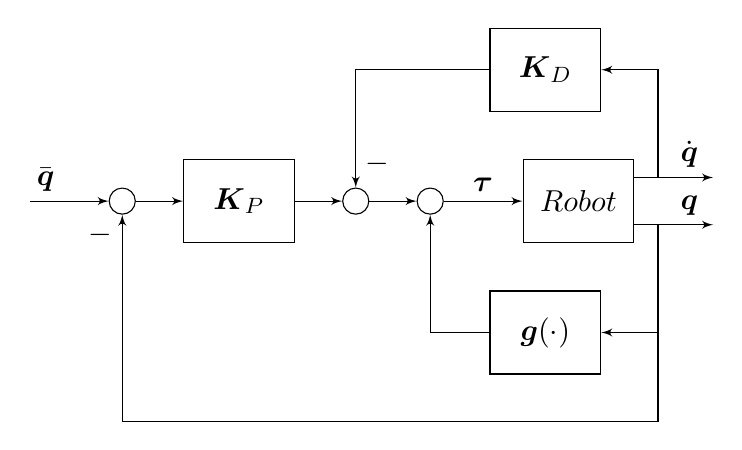
\begin{tikzpicture}
		\node [input] (iq_d) {};

		\node [sum, right=1cm of iq_d] (sum_e) {};
		\node [block, right=0.6cm of sum_e] (kp) {$\matr K_P$};
		\node [sum, right=0.6cm of kp] (sum_d) {};
		\node [sum, right=0.6cm of sum_d] (sum_g) {};
		\node [block, right=1cm of sum_g] (robot) {$Robot$};
		\node [block, above left=0.6cm and -1cm of robot] (kd) {$\matr K_D$};
		\node [block, below left=0.6cm and -1cm of robot] (g) {$\vect g(\cdot)$};

		\node [output, right=1cm of robot, yshift=0.3cm] (odq) {};
		\node [output, right=1cm of robot, yshift=-0.3cm] (oq) {};

		\draw [->] (iq_d) -- node[pos=0.2] {$\bar{\q}$} (sum_e);

		\draw [->] (sum_e) -- (kp);
		\draw [->] (kp) -- (sum_d);
		\draw [->] (sum_d) -- (sum_g);
		\draw [->] (sum_g) -- node {$\vect \tau$} (robot);

		\draw [->] (robot.east |- odq) -- node [pos=0.7] {$\dq$} node [spy, name=dq, pos=0.3] {}  (odq);
		\draw [->] (robot.east |- oq) -- node [pos=0.7] {$\q$} node [spy, name=q, pos=0.3] {} (oq);

		\draw [->] (q) |- (g);
		\draw [->] (g) -| (sum_g);

		\draw [->] (dq) |- (kd);
		\draw [->] (kd) -| node[pos=0.9] {$-$} (sum_d);
		\draw [->] (q) -- ++(0,-2.5) -| node[pos=0.95] {$-$} (sum_e);
	\end{tikzpicture}
	%}
	\caption{Closed loop with PD and gravity compensation}
	\label{fig:pd-gravity}
\end{figure}

\subsection{Inverse dynamics control}\label{subsec:inverse-dynamics-control-joints-space}

Let us try to solve the problem of the trajectory tracking.
we rewrite the \autoref{eq:simplified-dynamics} in the form

\[
	\matr{B}(\q)\ddq + \vect n(\q,\dq) = \vect \tau
\]

with

\[
	\vect n(\q,\dq) = \matr{C}(\q,\dq)\dq + \vect{g}(\q)
\]

If $\matr B(\q)$ is full rank for each configuration of the manipulator we can define the control law called \textbf{inverse dynamics}\index{inverse dynamics}

\begin{equation}
    \vect \tau = \matr{B}(\q)\vect y + \vect n(\q,\dq)\label{eq:control-law-inverse-dynamics-control-joints-space}
\end{equation}

so, if the system knowledge is perfect, this law impose the dynamics $\ddq = \vect y$;
from the extern the overall system appears as a double integrator.

Now we can design a control law for the function $\vect y$, a valid choice can be a \textbf{decoupled PD controller}\index{decoupled PD controller}

\begin{equation}
    \vect y = \matr K_P \qe + \matr K_I \dqe + \ddqd\label{eq:inverse-dynamics-control-law}
\end{equation}

that imposes the error dynamics

\[
	\ddqe + \matr K_D \dqe + \matr K_P \qe = 0
\]

then, the error $\qe$ is characterized by a second order dynamics that can be arbitrarily assigned by suitable choice of the parameters of the diagonal matrices $\matr K_P$ and $\matr K_I$.
This allows us to use this technique to track an assigned trajectory.

You can see the implementation of this control in \autoref{fig:inverse-dynamics-control}.

\begin{nb}this technique requires perfect knowledge of the dynamic model, which might be difficult in practice\end{nb}

\begin{figure}[htb]
	\centering
	\resizebox{\textwidth}{!}{
	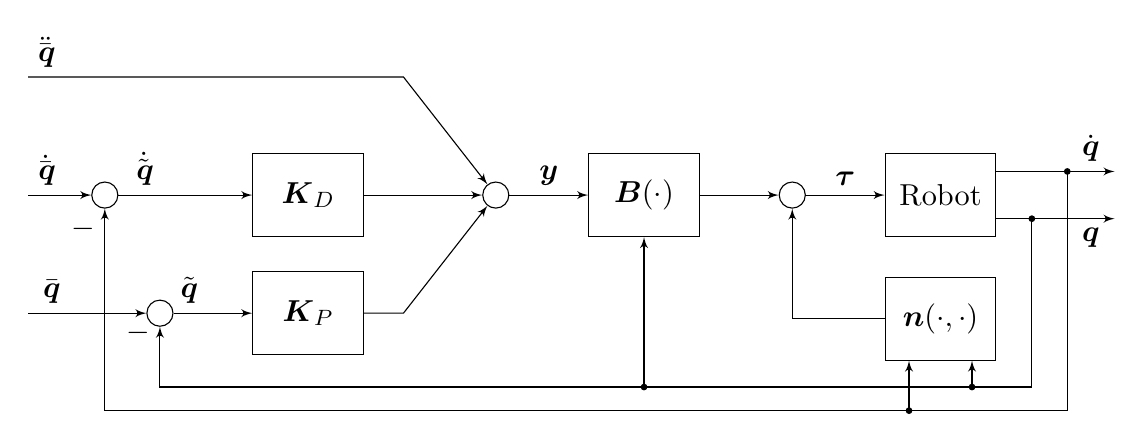
\begin{tikzpicture}
		\node [input] (iq_d) {};
		\node [input, above=1.5cm of iq_d] (idq_d) {};
		\node [input, above=1.5cm of idq_d] (iddq_d) {};

		\node [sum, right=1.5cm of iq_d] (sum_e) {};
		\node [sum, right=0.8cm of idq_d] (sum_de) {};

		\node [block, right=1cm of sum_e] (kp) {$\matr K_P$};
		\node [block] at (sum_de -| kp) (kd) {$\matr K_D$};

		\node [spy, right=0.5cm of kd] (bend) {};
		\node [sum, right=1.5cm of kd] (sum_y) {};

		\node [block, right=1cm of sum_y] (b) {$\matr B(\cdot)$};
		\node [sum, right=1cm of b] (sum_t) {};
		\node [block, right=1cm of sum_t] (robot) {Robot};

		\node [block, below=0.5cm of robot] (n) {$\vect n(\cdot,\cdot)$};

		\node [output, right=1.5cm of robot, yshift=0.3cm] (odq) {};
		\node [output, right=1.5cm of robot, yshift=-0.3cm] (oq) {};

		\node [node, below=0.3cm of n, xshift=0.4cm] (n_q) {};
		\node [node, below=0.6cm of n, xshift=-0.4cm] (n_dq) {};
		\node [node] at (n_q -| b) (b_q) {};

		\draw [->] (iq_d) -- node [pos=0.2] {$\qd$} (sum_e);
		\draw [->] (idq_d) -- node [pos=0.3] {$\dqd$} (sum_de);
		\draw [->] (iddq_d) -- node [pos=0.05] {$\ddqd$} (bend |- iddq_d) -- (sum_y);

		\draw [->] (sum_e) -- node [pos=0.2] {$\qe$} (kp);
		\draw [->] (sum_de) -- node [pos=0.2] {$\dqe$} (kd);

		\draw [->] (kp) -- (bend |- kp) -- (sum_y);
		\draw [->] (kd) -- (sum_y);

		\draw [->] (sum_y) -- node {$\vect y$} (b);
		\draw [->] (b) -- (sum_t);
		\draw [->] (sum_t) -- node {$\vect \tau$} (robot);

		\draw [->] (robot.east |- odq) -- node [pos=0.8] {$\dq$} node [node, name=dq, pos=0.6] {} (odq);
		\draw [->] (robot.east |- oq) -- node [pos=0.8, below] {$\q$} node [node, name=q, pos=0.3] {} (oq);

		\draw [->] (n) -| (sum_t);

		\draw [->] (q) |- (n_q) -- (b_q) -| node [pos=0.95] {$-$} (sum_e);
		\draw [->] (dq) |- (n_dq)  -| node [pos=0.95] {$-$} (sum_de);

		\draw [->] (n_q) -- (n_q |- n.south);
		\draw [->] (n_dq) -- (n_dq |- n.south);
		\draw [->] (b_q) -- (b_q |- b.south);
	\end{tikzpicture}
	}
	\caption{Closed loop with inverse dynamics control}
	\label{fig:inverse-dynamics-control}
\end{figure}

\subsubsection{Taking into account the uncertainty}\label{subsubsec:inverse-dynamics-robust-control}

As we saw in above the inverse dynamics control required perfect knowledge of the dynamics model of the robot, this is unrealistic in real robots, so we have to take into account the \textbf{model uncertainty}\index{model!uncertainty}.

Let us consider a more realist control law

\[
	\vect \tau = \Bs(\q) \vect y + \ns(\q,\dq)
\]

so the compensated system become

\[
	\B(\q)\ddq + \n(\q,\dq) = \Bs(\q) \y + \ns(\q,\dq)
\]

Let us define the \textbf{uncertainty} as

\[
	\Be(\q) = \Bs(\q) - \B(\q), \qquad
	\ner(\q,\dq) = \ns(\q, \dq) - \n(\q, \dq)
\]

still under the assumption that $\B(\q)$ is invertible, for $\ddq$ we can write

\[
	\ddq = \vect y - \vect \eta
\]

where

\[
	\vect\eta = \left( \I - \B^{-1} \Bs  \right)\y - \B^\inv \ner(\q,\dq)
\]

If we adopt the same control law we saw before in \autoref{eq:inverse-dynamics-control-law}, the error dynamic become

\[
	\ddqe + \matr K_D \dqe + \matr K_P \qe = \vect\eta
\]

the system still nonlinear, so we have to add in addiction to the PD controller a nonlinear term, function of the error to improve the robustness of the final system.

Let us define the second order derivative of the error

\[
	\ddqe = \ddqd - \ddq = \ddqd - \y + \vect \eta
\]

we define a new system whose state are the errors

\[
	\vect \xi = \begin{bmatrix} \qe^\trans \\ \dqe^\trans \end{bmatrix}
\]

and the dynamics is defined by

\[
	\dot{\vect\xi} = \matr H \vect\xi + \matr D \left( \ddqd - \y + \vect\eta \right)
\]

with

\[
	\matr H = \begin{bmatrix}\0&\I\\\0&\0\end{bmatrix} \in \mathbb{R}^{2n \times 2n}, \qquad
	\matr D = \begin{bmatrix}\0\\\I\end{bmatrix} \in \mathbb{R}^{2n \times n}
\]

Before we go any further, we need to characterize the uncertainty with three assumptions

\begin{itemize}
	\item $\sup_{t\ge0}\norm{\ddqd} < Q_M < \infty \qquad \forall \ddqd$

	This assumption requires that the required acceleration is not infinite.
	It is obviously always verified, because a planned trajectory will never require an unlimited acceleration.

	\item $\norm{\I - \B^\inv \Bs} \le \alpha < 1 \qquad \forall \q$

	A matrix $\B$ is definite positive and it is lower and upper bound, so the following equation is always valid
	\[ 0 < B_m \le \norm{\B^\inv} \le B_M < \infty \]
	then, we can impose
 	\[ \Bs = \frac{2}{B_M+B_m}\I \]
	that always satisfy the assumption
	\[ \norm{\I - \B^\inv \Bs} \le \frac{B_M-B_m}{B_M+B_m} < 1 \]
	\begin{nb}$\Bs = \B \implies \alpha = 0$\end{nb}

	\item $\norm{\ner} \le \Phi(\norm{\vect\xi}) < \infty \qquad \forall \q,\dq$

	We can choose the form
	\[ \Phi(\norm{\vect\xi}) = \alpha_0 + \alpha_1 \norm{\vect\xi} + \alpha_2 \norm{\vect\xi}^2 \]
\end{itemize}

We add a term to the control law \autoref{eq:inverse-dynamics-control-law}

\[
	\y = \K_P \qe + \K_I \dqe + \ddqd + \vect w
\]

now we consider the error dynamics with this control law

\begin{align*}
    \dot{\vect\xi} &= \matr H \vect\xi + \matr D \left(\vect\eta - \K_P \qe - \K_I \dqe - \vect w  \right) \\
	&= \tilde{\matr H} \vect\xi + \matr D \left(\vect\eta - \vect w \right)
\end{align*}

defining $\K = \begin{bmatrix}\K_P & \K_D\end{bmatrix}$ with

\[
	\tilde{\matr H} = (\matr H - \matr D \K) =
	\begin{bmatrix} \0&\I \\ - \K_P & \K_D \end{bmatrix}
\]

\begin{nb}all the eigenvalues of $\tilde{\matr H}$ are negative\end{nb}

Now, we need to design a control law for $\vect w$, and to do this we will use the \textbf{Lyapunov method}.
Consider the following \textbf{Lyapunov function} candidate

\[
	V(\vect\xi) = \vect\xi^\trans \matr Q \vect\xi > 0, \qquad \forall \vect\xi \div \vect 0
\]

where $\matr Q$ is symmetric positive definite matrix.

\begin{align*}
    \dot{V} &= \dot{\vect\xi}^\trans \matr Q \vect\xi + \vect\xi^\trans \matr Q \dot{\vect\xi} \\
    &= ( \vect\xi^\trans \tilde{\matr H}^\trans + \left(\vect\eta - \vect w \right)^\trans \matr D^\trans) \matr Q \vect\xi +
    \vect\xi^\trans \matr Q (\tilde{\matr H} \vect\xi + \matr D \left(\vect\eta - \vect w \right)) \\
	&= \vect\xi^\trans \left( \tilde{\matr H}^\trans \matr Q + \matr Q \tilde{\matr H} \right) \vect\xi +
    \left(\vect\eta - \vect w \right)^\trans \matr D^\trans \matr Q \vect\xi +
    \vect\xi^\trans \matr Q \matr D \left(\vect\eta - \vect w \right) \\
    \intertext{transposing the second element because it is a scalar}
	&= \vect\xi^\trans \left( \tilde{\matr H}^\trans \matr Q + \matr Q \tilde{\matr H} \right) \vect\xi +
    2 \vect\xi^\trans \matr Q \matr D \left(\vect\eta - \vect w \right)
    \intertext{set $\vect z = \matr D^\trans \matr Q \vect\xi$ and $\tilde{\matr H}^\trans \matr Q + \matr Q \tilde{\matr H} = -\matr P$}
    &= - \vect\xi^\trans \matr P \vect\xi +
    2 \vect z^\trans \left(\vect\eta - \vect w \right)
\end{align*}

\begin{nb}because all eigenvalues of $\tilde{\matr H}$ are negative for any $\matr P$ positive definite symmetrical matrix also the solution $\matr Q$ is a positive definite symmetrical matrix\end{nb}

Let us analyze the derivative Lyapunov function, the first element $- \vect\xi^\trans \matr P \vect\xi$ is always negative, so we need to analyze the second term.
If $\vect\xi \in \ker(\matr D^\trans \matr Q)$, then $\vect z = 0$, so the system is asymptotically stable, in the other case we have to define a control function $\vect w$ that make the second term negative.
From

\[
	\vect w = \rho \frac{\vect z}{\norm{\vect z}}
\]

we get

\[
	\vect z^\trans \left(\vect\eta - \vect w \right) =
	\vect z^\trans \left(\vect\eta - \rho \frac{\vect z}{\norm{\vect z}} \right) =
	\vect z^\trans \vect\eta - \rho \frac{\vect z^\trans \vect z}{\norm{\vect z}} \le \norm{\vect z}\norm{\vect\eta}-\rho\norm{\vect z} =
	\norm{\vect z}(\norm{\vect\eta} - \rho)
\]

so, if $\rho > \norm{\vect\eta}$ the globally asymptotically stability for the system is guaranteed.
Looking for define a function $\rho$ exploiting the assumptions

\begin{multline*}
    \norm{\vect\eta} \le
    	\norm{\I - \B^\inv \Bs} (\norm{\ddqd} + \norm{\K}\norm{\vect\xi} + \norm{\vect w} + \norm{\B^\inv}\norm{\ner}) \\
    	\le \alpha Q_M + \alpha \norm{\K} \norm{\vect\xi} + \alpha \rho + B_M \Phi(\norm{\vect\xi}) < \rho
\end{multline*}

so

\[
	\rho \ge \frac{1}{1-\alpha} \left(\alpha Q_M + \alpha \norm{\K} \norm{\vect\xi} + B_M \Phi(\norm{\vect\xi}) \right)
\]

under the assumption that $\Phi(\norm{\vect\xi})$ has the form $\alpha_0 + \alpha_1 \norm{\vect\xi} + \alpha_2 \norm{\vect\xi}^2$ we can chose

\[
	\rho(\norm{\vect \xi}) = \beta_0 + \beta_1 \norm{\vect\xi} + \beta_2 \norm{\vect\xi}^2
\]

with

\[
	\beta_0 \ge \frac{\alpha Q_M + \alpha_0 B_M}{1 - \alpha}, \qquad
	\beta_1 \ge \frac{\alpha \norm{\K} + \alpha_1 B_M}{1 - \alpha}, \qquad
	\beta_2 \ge \frac{\alpha_2 B_M}{1 - \alpha}
\]

this control law guarantees a globally asymptotically stability of the system.

So the overall control law is composed by three terms

\begin{itemize}
	\item $\Bs(\q)\y + \ns(\q,\dq)$ \\
	approximately compensated for the nonlinear terms

	\item $\K_P\qe + \K_D\dqe + \ddqd$ \\
	stabilizes the nominal dynamic system in the error

	\item $\vect w = \rho(\norm{\vect \xi}) \frac{\vect z}{\norm{\vect z}}$ \\
	gives robustness, counteracting the uncertainty
\end{itemize}

A further improvement can be done, in order to avoid high frequency switching of the control variable, called \textbf{chattering}\index{chattering}, the third term can be changed to

\[
	\vect w =
	\begin{cases}
		\rho(\norm{\vect \xi}) \frac{\vect z}{\norm{\vect z}} & \norm{\vect z} \ge \epsilon \\
		\rho(\norm{\vect \xi}) \frac{\vect z}{\epsilon} & \norm{\vect z} < \epsilon
	\end{cases}
\]

\begin{figure}[htb]
	\centering
	\resizebox{\textwidth}{!}{
	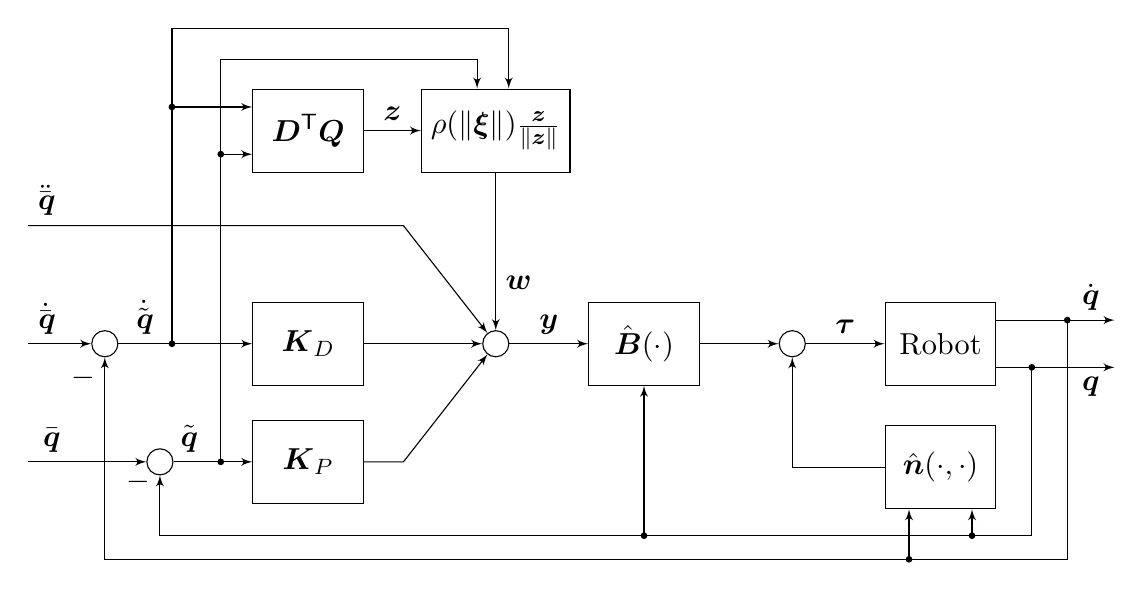
\begin{tikzpicture}
		\node [input] (iq_d) {};
		\node [input, above=1.5cm of iq_d] (idq_d) {};
		\node [input, above=1.5cm of idq_d] (iddq_d) {};

		\node [sum, right=1.5cm of iq_d] (sum_e) {};
		\node [sum, right=0.8cm of idq_d] (sum_de) {};

		\node [block, right=1cm of sum_e] (kp) {$\matr K_P$};
		\node [block] at (sum_de -| kp) (kd) {$\matr K_D$};

		\node [spy, right=0.5cm of kd] (bend) {};
		\node [sum, right=1.5cm of kd] (sum_y) {};

		\node [block, right=1cm of sum_y] (b) {$\hat{\matr B}(\cdot)$};
		\node [sum, right=1cm of b] (sum_t) {};
		\node [block, right=1cm of sum_t] (robot) {Robot};

		\node [block, below=0.5cm of robot] (n) {$\hat{\vect n}(\cdot,\cdot)$};

		\node [output, right=1.5cm of robot, yshift=0.3cm] (odq) {};
		\node [output, right=1.5cm of robot, yshift=-0.3cm] (oq) {};

		\node [node, below=0.3cm of n, xshift=0.4cm] (n_q) {};
		\node [node, below=0.6cm of n, xshift=-0.4cm] (n_dq) {};
		\node [node] at (n_q -| b) (b_q) {};

		\draw [->] (iq_d) -- node [pos=0.2] {$\qd$} (sum_e);
		\draw [->] (idq_d) -- node [pos=0.3] {$\dqd$} (sum_de);
		\draw [->] (iddq_d) -- node [pos=0.05] {$\ddqd$} (bend |- iddq_d) -- (sum_y);

		\draw [->] (sum_e) -- node [pos=0.2] {$\qe$} node[node, pos=0.6] (qe) {} (kp);
		\draw [->] (sum_de) -- node [pos=0.2] {$\dqe$} node[node, pos=0.4] (dqe) {} (kd);

		\draw [->] (kp) -- (bend |- kp) -- (sum_y);
		\draw [->] (kd) -- (sum_y);

		\draw [->] (sum_y) -- node {$\vect y$} (b);
		\draw [->] (b) -- (sum_t);
		\draw [->] (sum_t) -- node {$\vect \tau$} (robot);

		\draw [->] (robot.east |- odq) -- node [pos=0.8] {$\dq$} node [node, name=dq, pos=0.6] {} (odq);
		\draw [->] (robot.east |- oq) -- node [pos=0.8, below] {$\q$} node [node, name=q, pos=0.3] {} (oq);

		\draw [->] (n) -| (sum_t);

		\draw [->] (q) |- (n_q) -- (b_q) -| node [pos=0.95] {$-$} (sum_e);
		\draw [->] (dq) |- (n_dq)  -| node [pos=0.95] {$-$} (sum_de);

		\draw [->] (n_q) -- (n_q |- n.south);
		\draw [->] (n_dq) -- (n_dq |- n.south);
		\draw [->] (b_q) -- (b_q |- b.south);

		\node [block, above=2cm of sum_y] (w) {$\rho(\norm{\vect\xi})\frac{\vect z}{\norm{\vect z}}$};
		\node [block] at (kd |- w) (t) {$\matr D^\trans \matr Q$};

		\node [node, yshift=0.3cm] at (dqe |- t) (dqe_t) {};
		\node [node, yshift=-0.3cm] at (qe |- t) (qe_t) {};

		\draw [->] (qe) -- (qe_t) -- ++(0,1.2) -| ([xshift=-0.4cm]w);
		\draw [->] (dqe) -- (dqe_t) -- ++(0,1.0) -| ([xshift=0.4cm]w);

		\draw [->] (qe_t) -- (qe_t -| t.west);
		\draw [->] (dqe_t) -- (dqe_t -| t.west);

		\draw [->] (t) -- node {$\vect z$} (w);
		\draw [->] (w) -- node[pos=0.7] {$\vect w$} (sum_y);

	\end{tikzpicture}
	}

	\caption{Closed loop with inverse dynamics robust control}
	\label{fig:inverse-dynamics-robust-control}
\end{figure}

\subsubsection{Adaptive control}

In additional to the inverse dynamics robust control (\autoref{subsubsec:inverse-dynamics-robust-control}) we can consider an adaptive control to compensate the \text{uncertain dynamic parameters}\index{uncertain dynamic parameters}.
As we saw in \autoref{subsec:linearity-in-dynamic-parameters}  the dynamic model can write as

\[
	\matr{B}(\q)\ddq + \matr{C}(\q,\dq)\dq + \vect{g}(\q) = \matr Y(\q,\dq,\ddq)\vect\pi = \vect\tau
\]

where $\vect\pi$ is a suitable constant vector of \text{uncertain dynamic parameters}.

Let us consider the control law

\[
	\vect\tau = \matr{B}(\q)\ddq_r + \matr{C}(\q,\dq)\dq_r + \vect{g}(\q) + \K_D\vect\sigma
\]

where

\[
	\dq_r = \dqd + \matr\Lambda \qe \qquad \ddq_r = \ddqd + \matr\Lambda \dqe
\]

with $\matr\Lambda$ symmetrical positive define matrix (usually diagonal).
If we impose

\[
	\vect\sigma = \dq_r - \dq = \dqe + \matr\Lambda\qe
\]

we get as overall system

\begin{align}
    \matr{B}(\q)\ddq + \matr{C}(\q,\dq)\dq + \vect{g}(\q) &= \matr{B}(\q)\ddq_r + \matr{C}(\q,\dq)\dq_r + \vect{g}(\q) + \K_D \vect\sigma \nonumber \\
    \matr{B}(\q)\ddq + \matr{C}(\q,\dq)\dq  &= \matr{B}(\q)\ddq_r + \matr{C}(\q,\dq)\dq_r + \K_D \vect\sigma \nonumber \\
    \matr{B}(\q) \left( \ddq - \ddq_r \right) + \matr{C}(\q,\dq) \left( \dq - \dq_r \right) &= \K_D \vect\sigma \nonumber \\
    - \matr{B}(\q) \dot{\vect\sigma} - \matr{C}(\q,\dq) \vect\sigma &= \K_D \vect\sigma \nonumber \\
    \matr{B}(\q) \dot{\vect\sigma} + \matr{C}(\q,\dq) \vect\sigma + \K_D \vect\sigma &= \0 \label{eq:adaptive-control-sigma-dynamics}
\end{align}

So let us check the stability of this system using the Lyapunov function

\[
	V(\vect\sigma, \qe) = \frac{1}{2} \vect\sigma^\trans \B(\q) \vect\sigma + \frac{1}{2} \qe^\trans \matr M \qe
\]

$\matr M$ is (as always) a positive definite matrix, so the derivative is

\begin{align*}
    \dot{V} &= \vect\sigma^\trans \B(\q) \dot{\vect\sigma} + \frac{1}{2} \vect\sigma^\trans \dB(\q) \vect\sigma + \qe^\trans \matr M \dqe \\
    \intertext{using $\B(\q) \dot{\vect\sigma}$ from \autoref{eq:adaptive-control-sigma-dynamics}}
	&= \vect\sigma^\trans \left( - \matr{C}(\q,\dq)  - \K_D \right) \vect\sigma + \frac{1}{2} \vect\sigma^\trans \dB(\q) \vect\sigma + \qe^\trans \matr M \dqe \\
	&= - \vect\sigma^\trans \K_D \vect\sigma + \frac{1}{2} \vect\sigma^\trans \left( \dB(\q) - 2 \matr{C}(\q,\dq)\right) \vect\sigma + \qe^\trans \matr M \dqe \\
    \intertext{remembering the property of the matrix  $\dB(\q) - 2 \matr{C}(\q,\dq)$ seen in \autoref{subsec:matrix-db-2c}}
    &= - \vect\sigma^\trans \K_D \vect\sigma + \qe^\trans \matr M \dqe \\
	&= -(\dqe + \matr\Lambda\qe)^\trans \K_D (\dqe + \matr\Lambda\qe) + \qe^\trans \matr M \dqe \\
	&= - \dqe^\trans \K_D \dqe - \qe^\trans \matr\Lambda \K_D \matr\Lambda\qe - 2 \qe^\trans \matr\Lambda \K_D \dqe + \qe^\trans \matr M \dqe \\
	\intertext{choosing $\matr M = 2 \matr\Lambda \K_D$}
    &= - \dqe^\trans \K_D \dqe - \qe^\trans \matr\Lambda \K_D \matr\Lambda\qe \\
\end{align*}

$\dot{V}$ is negative define thus the system is globally asymptotically stable with the equilibrium $\qe = 0, \dqe = 0 $

Now let us consider a control law where the parameters are estimated and exploiting the formulation with the parametric vector we saw above

\begin{align*}
    \vect\tau &= \Bs(\q)\ddq_r + \Cs(\q,\dq)\dq_r + \gs(\q) + \K_D\vect\sigma \\
    &= \matr Y (\q,\dq,\dq_r,\ddq_r)\estimate{\vect\pi} + \K_D\vect\sigma
\end{align*}

the system dynamic model \autoref{eq:adaptive-control-sigma-dynamics} become

\begin{align*}
    \B(\q) \dot{\vect\sigma} + \matr{C}(\q,\dq) \vect\sigma + \K_D \vect\sigma &=
    - \Be(\q) \ddq_r - \Ce(\q,\dq) \dq_r - \error\g(\q) \\
    &= - \matr Y (\q,\dq,\dq_r,\ddq_r)\error{\vect\pi}
\end{align*}

where $\Be, \Ce, \error\g$ are the residual error given by the estimate of the model parameters, and thus the $\matr Y (\q,\dq,\dq_r,\ddq_r)\error{\vect\pi}$ can be seen as the model residual error.

So consider a modified version of the Lyapunov function saw before

\[
	V(\vect\sigma, \qe, \error{\vect\pi}) = \frac{1}{2} \vect\sigma^\trans \B(\q) \vect\sigma + \qe^\trans \matr\Lambda \K_D \qe + \frac{1}{2} \error{\vect\pi}^\trans \K_\pi \error{\vect\pi}
\]

where $\matr M$ is already substituted and $\K_\pi$ is a positive define matrix

\begin{align*}
    \dot V &= \vect\sigma^\trans \B(\q) \dot{\vect\sigma} + \frac{1}{2} \vect\sigma^\trans \dB(\q) \vect\sigma +
    2 \qe^\trans \matr\Lambda \K_D \dqe + \error{\vect\pi}^\trans \K_\pi \dot{\error{\vect\pi}} \\
    \intertext{using $\B(\q) \dot{\vect\sigma}$ from uncertain dynamics model}
    &= \vect\sigma^\trans \left( - \matr{C}(\q,\dq)  - \K_D \right) \vect\sigma - \vect\sigma^\trans \matr Y (\q,\dq,\dq_r,\ddq_r)\error{\vect\pi}
    + \frac{1}{2} \vect\sigma^\trans \dB(\q) \vect\sigma \\ & \hspace{0.6\textwidth}
    + 2 \qe^\trans \matr\Lambda \K_D \dqe + \error{\vect\pi}^\trans \K_\pi \dot{\error{\vect\pi}} \\
    &= - \vect\sigma^\trans \K_D \vect\sigma + \frac{1}{2} \vect\sigma^\trans \left( \dB(\q) - 2 \matr{C}(\q,\dq)\right) \vect\sigma
    - \vect\sigma^\trans \matr Y (\q,\dq,\dq_r,\ddq_r)\error{\vect\pi}  \\ & \hspace{0.6\textwidth}
    + 2 \qe^\trans \matr\Lambda \K_D \dqe + \error{\vect\pi}^\trans \K_\pi \dot{\error{\vect\pi}} \\
    &= - \vect\sigma^\trans \K_D \vect\sigma
    - \vect\sigma^\trans \matr Y (\q,\dq,\dq_r,\ddq_r)\error{\vect\pi} + 2 \qe^\trans \matr\Lambda \K_D \dqe + \error{\vect\pi}^\trans \K_\pi \dot{\error{\vect\pi}} \\
    &= - \vect\sigma^\trans \K_D \vect\sigma
     + 2 \qe^\trans \matr\Lambda \K_D \dqe + \error{\vect\pi}^\trans (\K_\pi \dot{\error{\vect\pi}} -  \matr Y^\trans (\q,\dq,\dq_r,\ddq_r) \vect\sigma) \\
    \intertext{using $\vect\sigma$}
    &= - (\dqe + \matr\Lambda\qe)^\trans \K_D (\dqe + \matr\Lambda\qe)
    + 2 \qe^\trans \matr\Lambda \K_D \dqe + \error{\vect\pi}^\trans (\K_\pi \dot{\error{\vect\pi}} -  \matr Y^\trans (\q,\dq,\dq_r,\ddq_r) \vect\sigma) \\
	&= - \dqe^\trans \K_D \dqe - \qe^\trans \matr\Lambda \K_D \matr\Lambda \qe - 2 \qe^\trans \matr\Lambda \K_D \dqe
    + 2 \qe^\trans \matr\Lambda \K_D \dqe \\ & \hspace{0.5\textwidth}
    + \error{\vect\pi}^\trans (\K_\pi \dot{\error{\vect\pi}} -  \matr Y^\trans (\q,\dq,\dq_r,\ddq_r) \vect\sigma) \\
    &= - \dqe^\trans \K_D \dqe - \qe^\trans \matr\Lambda \K_D \matr\Lambda \qe
    + \error{\vect\pi}^\trans (\K_\pi \dot{\error{\vect\pi}} -  \matr Y^\trans (\q,\dq,\dq_r,\ddq_r) \vect\sigma) \\
	\intertext{if we update the parameters' estimate as $\dot{\estimate{\vect\pi}}=\K_\pi^\inv \matr Y^\trans (\q,\dq,\dq_r,\ddq_r) \vect\sigma=\dot{\error{\vect\pi}}$}
    &= - \dqe^\trans \K_D \dqe - \qe^\trans \matr\Lambda \K_D \matr\Lambda \qe
\end{align*}

$\dot{V} < 0$ thus, the system is globally asymptotically stable with the equilibrium $\qe = 0, \dqe = 0$

So, in summary the overall control law (which you can see in the \autoref{fig:adaptive-control}) is described by the system

\begin{align*}
	\dot{\estimate{\vect\pi}} &= \K_\pi^\inv \matr Y^\trans (\q,\dq,\dq_r,\ddq_r) (\dqe + \matr\Lambda\qe) \\
	\vect\tau &= \matr Y (\q,\dq,\dq_r,\ddq_r)\estimate{\vect\pi} + \K_D (\dqe + \matr\Lambda\qe) \\
\end{align*}

in which we can identify three terms

\begin{itemize}
	\item $\matr Y (\q,\dq,\dq_r,\ddq_r)\estimate{\vect\pi}$ \\
	can be interpreted as an approximate inverse dynamic control

	\item $\K_D (\dqe + \matr\Lambda\qe)$ \\
	has the behaviour of a PD acting on the tracking error

	\item $\K_\pi^\inv \matr Y^\trans (\q,\dq,\dq_r,\ddq_r) (\dqe + \matr\Lambda\qe)$ \\
	update the estimate of parameters in according to a gradient technique.
	The matrix $\K_\pi$ defines the speed of the convergence of the estimate to its asymptotic value.
\end{itemize}

\begin{nb}asymptotically we will not get $\estimate{\vect\pi} \to \vect\pi$, but only $\matr Y(\q,\dq,\dq_r,\ddq_r)(\estimate{\vect\pi} - \vect\pi) \to \0$\end{nb}

\begin{figure}[htb]
	\centering
	\resizebox{\textwidth}{!}{
		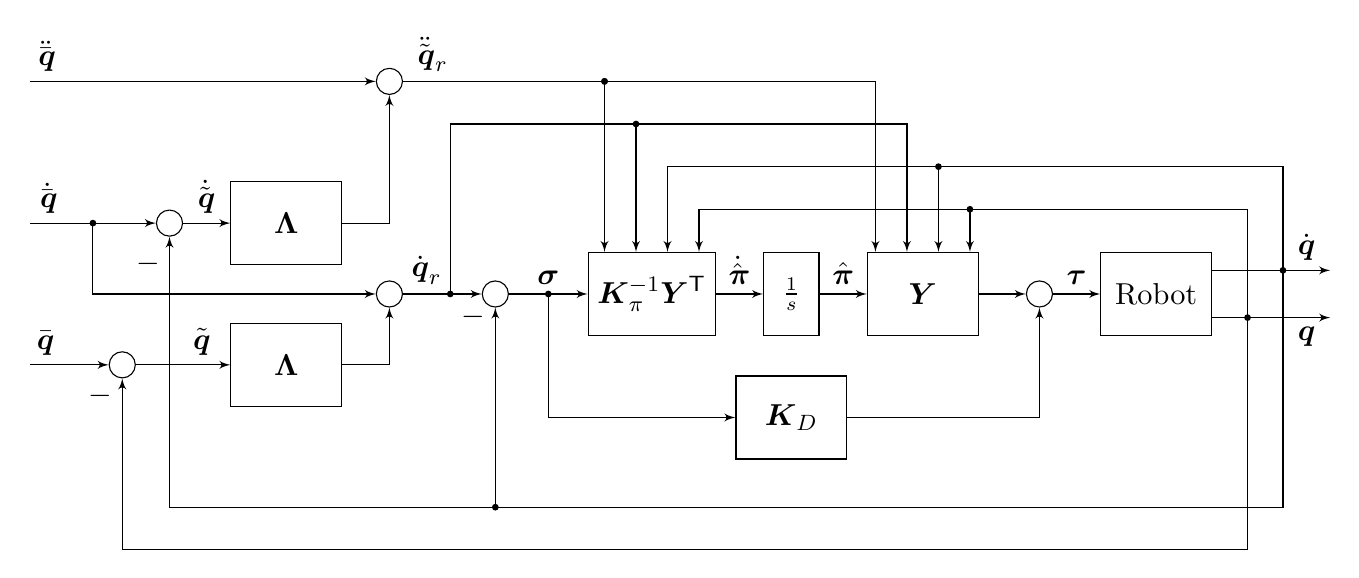
\begin{tikzpicture}
			\node [input] (iq_d) {};
			\node [input, above=1.8cm of iq_d] (idq_d) {};
			\node [input, above=1.8cm of idq_d] (iddq_d) {};

			\node [sum, right=1cm of iq_d] (sum_e) {};
			\node [sum, xshift=0.6cm] at (idq_d -| sum_e) (sum_de) {};
			\node [block, right=0.6cm of sum_de] (lambda_de) {$\matr\Lambda$};
			\node [block] at (sum_e -| lambda_de) (lambda_e) {$\matr\Lambda$};

			\node [sum, xshift=0.6cm] at ($(lambda_e.east)!0.5!(lambda_de.east)$) (sum_dqr) {};
			\node [sum] at (iddq_d -| sum_dqr) (sum_ddqr) {};

			\node [sum, right=1cm of sum_dqr] (sum_s) {};

			\node [block, right=1cm of sum_s] (s2dpis) {$\K_\pi^\inv \matr Y^\trans$};
			\node [integrator, right=0.6cm of s2dpis] (dpis2pis) {};
			\node [block, right=0.6cm of dpis2pis] (y) {$\matr Y$};

			\node [block, below=0.5cm of dpis2pis] (kd) {$\K_D$};

			\node [sum, right=0.6cm of y] (sum_t) {};
			\node [block, right=0.6cm of sum_t] (robot) {Robot};

			\node [output, right=1.5cm of robot, yshift=0.3cm] (odq) {};
			\node [output, right=1.5cm of robot, yshift=-0.3cm] (oq) {};

			\draw [->] (iq_d) -- node[pos=0.2] {$\qd$} (sum_e);
			\draw [->] (idq_d) -- node[pos=0.15] {$\dqd$} node[node, name=dqd, pos=0.5] {} (sum_de);
			\draw [->] (iddq_d) -- node[pos=0.05] {$\ddqd$} (sum_ddqr);
			\draw [->] (dqd) |- (sum_dqr);

			\draw [->] (sum_dqr) -- node[node, name=dqr, pos=0.6] {} node[pos=0.3] {$\dq_r$} (sum_s);
			\draw [->] (sum_s) -- node[node, name=s] {} node {$\vect\sigma$} (s2dpis);

			\draw [->] (s2dpis) -- node {$\dot{\estimate{\vect\pi}}$} (dpis2pis);
			\draw [->] (dpis2pis) -- node {$\estimate{\vect\pi}$} (y);
			\draw [->] (y) -- (sum_t);

			\draw [->] (s) |- (kd);
			\draw [->] (kd) -| (sum_t);

			\draw [->] (sum_t) -- node {$\vect\tau$} (robot);

			\draw [->] (robot.east |- odq) -- node [pos=0.8] {$\dq$} node [node, name=dq, pos=0.6] {} (odq);
			\draw [->] (robot.east |- oq) -- node [pos=0.8, below] {$\q$} node [node, name=q, pos=0.3] {} (oq);

			\draw [->] (sum_e) -- node[pos=0.7] {$\qe$} (lambda_e);
			\draw [->] (lambda_e) -| (sum_dqr);

			\draw [->] (sum_de) -- node {$\dqe$} (lambda_de);

			\draw [->] (lambda_de) -| (sum_ddqr);

			\node [node, below=2.5cm of sum_s] (dq_f) {};
			\node [spy, below=0.5cm of dq_f] (q_f) {};

			\draw [->] (dq) |- (dq_f)  -| node[pos=0.95] {$-$} (sum_de);
			\draw [->] (dq_f) -- node[pos=0.95] {$-$} (sum_s);
			\draw [->] (q) |- (q_f)  -| node[pos=0.95] {$-$} (sum_e);


			\node [node] at ([xshift=-0.6cm]iddq_d -| s2dpis) (s2dpis_ddqr2) {};
			\node [node] at ([xshift=-0.6cm]$(s2dpis.north |- iddq_d)!0!(s2dpis.north)$) (ddqr_1) {};
			\node [node] at ([xshift=-0.2cm]$(s2dpis.north |- iddq_d)!0.25!(s2dpis.north)$) (dqr_1) {};
			\node [spy] at ([xshift=0.2cm]$(s2dpis.north |- iddq_d)!0.5!(s2dpis.north)$) (dq_2) {};
			\node [spy] at ([xshift=0.6cm]$(s2dpis.north |- iddq_d)!0.75!(s2dpis.north)$) (q_2) {};

			\node [spy] at ([xshift=-0.6cm]$(y.north |- iddq_d)!0!(y.north)$) (ddqr_2) {};
			\node [spy] at ([xshift=-0.2cm]$(y.north |- iddq_d)!0.25!(y.north)$) (dqr_2) {};
			\node [node] at ([xshift=0.2cm]$(y.north |- iddq_d)!0.5!(y.north)$) (dq_1) {};
			\node [node] at ([xshift=0.6cm]$(y.north |- iddq_d)!0.75!(y.north)$) (q_1) {};

			\draw [->] (q) |- (q_1) -- (y.north -| q_1);
			\draw [->] (dq) |- (dq_1) -- (y.north -| dq_1);
			\draw [->] (q_1) -- (q_2) -- (y.north -| q_2);
			\draw [->] (dq_1) -- (dq_2) -- (y.north -| dq_2);

			\draw [->] (sum_ddqr) -- node[pos=0.15] {$\ddqe_r$} (ddqr_1) -- (s2dpis.north -| ddqr_1);
			\draw [->] (dqr) |- (dqr_1) -- (s2dpis.north -| dqr_1);
			\draw [->] (ddqr_1) -- (ddqr_2) -- (y.north -| ddqr_2);
			\draw [->] (dqr_1) -- (dqr_2) -- (y.north -| dqr_2);
		\end{tikzpicture}
	}

	\caption{Adaptive control scheme}
	\label{fig:adaptive-control}
\end{figure}

In conclusion the \textbf{adaptive control} offers worse performance than the \textbf{robust control} in presence of model errors, but this first guarantees a more regular control action than the \textbf{robust control}, which are characterized by potentially dangerous high frequency switching.


\section{Control in operational space}

In opposite to the control in the joints space, we can implement the control directly in the operational space (a Cartesian space).

As first difference by the control in the joints space, we will not apply the kinematic inversion, but the measures are actually the result of the direct kinematics computations based (generally) on the joint measures.

\subsection{PD + gravity compensation}

In a cartesian space we can define the error as

\[
	\xe = \xd - \x
\]

Let us consider a Lyapunov function

\[
	V(\xe,\dq) = \frac{1}{2} \dq^\trans\B(\q)\dq + \frac{1}{2}\xe^\trans \K_P \xe
\]

with $\K_P$ symmetric positive definite matrix

\begin{align*}
    \dot V &= \dq^\trans \B(\q) \ddq + \frac{1}{2} \dq^\trans \dB(\q) \dq + \dxe^\trans \matr K_P \xe \\
	\intertext{exploiting the \textbf{analytic Jacobian}\index{analytic Jacobian} we have $\dxe=\dx=-\J_A(\q)\dq$}
	&= \dq^\trans \B(\q) \ddq + \frac{1}{2} \dq^\trans \dB(\q) \dq - \dq^\trans \J_A^\trans(\q)\K_P \xe \\
    \intertext{replacing $\B\ddq$ with the \autoref{eq:simplified-dynamics}}
	&= \dq^\trans \left( \vect\tau - \C(\q,\dq)\dq - \g(\q) \right) + \frac{1}{2} \dq^\trans \dB(\q) \dq - \dq^\trans \J_A^\trans(\q)\K_P \xe \\
	&= \frac{1}{2} \dq^\trans \left(\dB(\q) - 2\C(\q,\dq) \right) \dq + \dq^\trans \left( \vect\tau - \g(\q)  - \J_A^\trans(\q)\K_P \xe \right) \\
	\intertext{with the property we saw in \autoref{subsec:matrix-db-2c} we can eliminate the first term}
	&= \dq^\trans \left( \vect\tau - \g(\q)  - \J_A^\trans(\q)\K_P \xe \right) \\
    \intertext{consider the control law $\vect\tau = \g(\q) + \J_A^\trans(\q) \K_P \xe - \J_A^\trans(\q) \K_D \J_A(\q) \dq$}
	&= \dq^\trans \left( \g(\q) + \J_A^\trans(\q) \K_P \xe - \J_A^\trans(\q) \K_D \J_A(\q) \dq - \g(\q)  - \J_A^\trans(\q)\K_P \xe \right) \\
	&= - \dq^\trans \J_A^\trans(\q) \K_D \J_A(\q) \dq
\end{align*}

we can state $\dot V \le 0$ ($\dot V = 0$ for $\dq=0, \forall \xe \in \Real $) so let us check the system trajectory.
The dynamics model (\autoref{eq:simplified-dynamics}) with the control law become

\[
	\matr{B}(\q)\ddq + \matr{C}(\q,\dq)\dq = \J_A^\trans(\q) \K_P \xe - \J_A^\trans(\q) \K_D \J_A(\q) \dq
\]

evaluated in the equilibrium $\dq = 0, \ddq = 0$

\[
	\J_A^\trans(\q) \K_P \xe = \0
\]

so, if the Jacobian is full rank the only solution is $\xe = 0$, thus the system is globally asymptotically stable with the equilibrium $\xd = \x$.
You can see the corresponding scheme in \autoref{fig:pd-gravity-operational}

\begin{figure}[htb]
	\centering
	%\resizebox{\textwidth}{!}{
	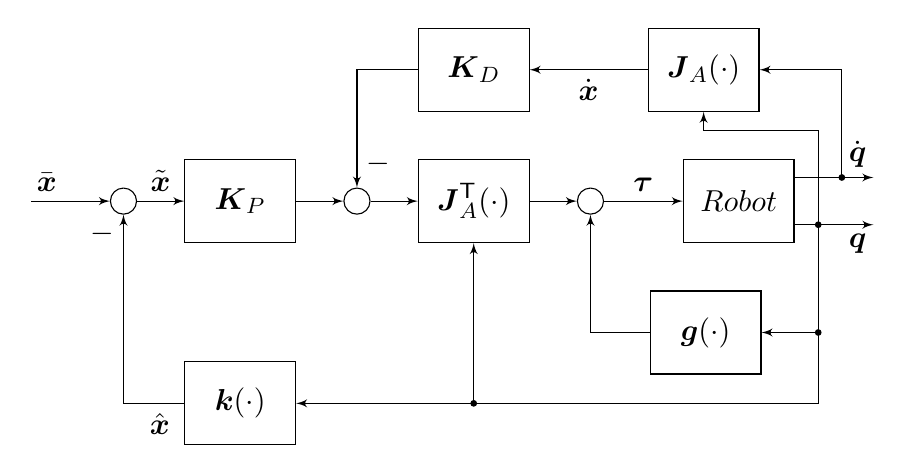
\begin{tikzpicture}
		\node [input] (iq_d) {};

		\node [sum, right=1cm of iq_d] (sum_e) {};
		\node [block, right=0.6cm of sum_e] (kp) {$\matr K_P$};
		\node [sum, right=0.6cm of kp] (sum_d) {};
		\node [block, right=0.6cm of sum_d] (ja_t) {$\J_A^\trans(\cdot)$};
		\node [sum, right=0.6cm of ja_t] (sum_g) {};
		\node [block, right=1cm of sum_g] (robot) {$Robot$};
		\node [block, above=0.6cm of ja_t] (kd) {$\matr K_D$};
		\node [block, right=1.5cm of kd] (ja) {$\J_A(\cdot)$};
		\node [block, below left=0.6cm and -1cm of robot] (g) {$\vect g(\cdot)$};

		\node [output, right=1cm of robot, yshift=0.3cm] (odq) {};
		\node [output, right=1cm of robot, yshift=-0.3cm] (oq) {};

		\node [block, below=1.5cm of kp] (k) {$\vect k(\cdot)$};


		\node [node] at (k -| ja_t) (q_f) {};

		\draw [->] (iq_d) -- node[pos=0.2] {$\xd$} (sum_e);

		\draw [->] (sum_e) -- node {$\xe$} (kp);
		\draw [->] (kp) -- (sum_d);
		\draw [->] (sum_d) -- (ja_t);
		\draw [->] (ja_t) -- (sum_g);
		\draw [->] (sum_g) -- node {$\vect \tau$} (robot);

		\draw [->] (robot.east |- odq) -- node [pos=0.8] {$\dq$} node [node, name=dq, pos=0.6] {} (odq);
		\draw [->] (robot.east |- oq) -- node [pos=0.8, below] {$\q$} node [node, name=q, pos=0.3] {} (oq);

		\node [node] at (q |- g) {};
		\draw [->] (q |- g) -- (g);
		\draw [->] (g) -| (sum_g);

		\draw [->] (q) -- +(0,1.2) -| (ja);

		\draw [->] (dq) |- (ja);
		\draw [->] (ja) -- node {$\dx$} (kd);
		\draw [->] (kd) -| node[pos=0.9] {$-$} (sum_d);
		\draw [->] (k) -| node[pos=0.2] {$\xs$} node[pos=0.95] {$-$} (sum_e);

		\draw [->] (q) |- (k);
		\draw [->] (q_f) -- (ja_t);
	\end{tikzpicture}
	%}
	\caption{PD and gravity compensation in the operational space}
	\label{fig:pd-gravity-operational}
\end{figure}

\subsection{Inverse dynamics control}

To tracking a trajectory the \textbf{PD + gravity compesation} is not usable (it is constrained by $\dxd = 0$), so we have to implement a different control system, in particular we can adapt the \textbf{inverse dynamics control} designed to the control in the \textbf{joints space} saw in \autoref{subsec:inverse-dynamics-control-joints-space}.

As we saw if we impose the control law in \autoref{eq:control-law-inverse-dynamics-control-joints-space} we get that $\ddq = \y$, so we have to design a new input $\y$ in such a way to allow the trackinf of the trajectory $\xd(t)$.
A way to do this is notice that

\[
	\ddx = \frac{d}{dt} \dx = \frac{d}{dt} \left( \J_A(\q)\dq \right) = \J_A(\q)\ddq + \dJ_A(\q,\dq)\dq
\]

so we can invert the function and get

\[
	\ddq = \J_A^\inv(\q) \left(\ddx - \dJ_A(\q,\dq)\dq\right)
\]

this suggests that a possible control law for $\y$ can be

\[
	\y = \J_A^\inv(\q) \left( \ddxd + \K_D\dxe + \K_P \xe - \dJ_A(\q,\dq)\dq \right)
\]

so the overall control law become

\[
	\vect\tau = \B(\q) \J_A^\inv(\q) \left( \ddxd + \K_D\dxe + \K_P \xe - \dJ_A(\q,\dq)\dq \right) + \vect n(\q,\dq)
\]

Let us find the error dynamics beginning from the dynamic model subject the above control law

\begin{align*}
    \matr{B}(\q)\ddq + \vect n(\q,\dq) &= \B(\q) \J_A^\inv(\q) \left( \ddxd + \K_D\dxe + \K_P \xe - \dJ_A(\q,\dq)\dq \right) + \vect n(\q,\dq) \\
    \matr{B}(\q)\ddq &= \B(\q) \J_A^\inv(\q) \left( \ddxd + \K_D\dxe + \K_P \xe - \dJ_A(\q,\dq)\dq \right) \\
    \0 &= \ddxd + \K_D\dxe + \K_P \xe - \dJ_A(\q,\dq)\dq - \J_A(\q) \ddq \\
    \intertext{substitute $\ddq$}
    \0 &= \ddxd + \K_D\dxe + \K_P \xe - \dJ_A(\q,\dq)\dq - \ddx - \dJ_A(\q,\dq)\dq \\
    \0 &= \ddxd + \K_D\dxe + \K_P \xe - \ddx \\
    \intertext{recognize $\ddxe = \ddxd - \ddx$}
    \0 &= \ddxe + \K_D\dxe + \K_P \xe \\
\end{align*}

So the dynamics of the error in the operative space is characterized by a second order function with  $\K_P, \K_D$ arbitrarly assigned.
You can see the schema in \autoref{fig:inverse-dynamics-control-operational-space}.

\begin{nb}to compute the control law we have to invert the Jacobian $\J_A^\inv$, thus this method can not been used for the control of the \textbf{redundant robots} or for robots in \textbf{singular configurations}\end{nb}


\begin{figure}[htb]
	\centering
	\resizebox{\textwidth}{!}{
		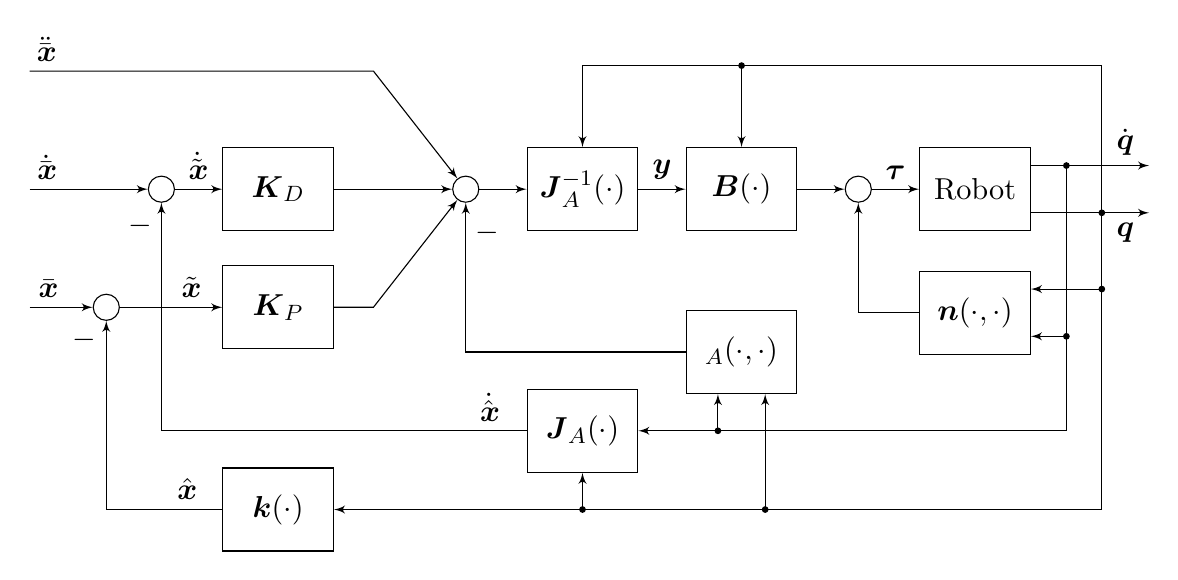
\begin{tikzpicture}
			\node [input] (iq_d) {};
			\node [input, above=1.5cm of iq_d] (idq_d) {};
			\node [input, above=1.5cm of idq_d] (iddq_d) {};

			\node [sum, right=0.8cm of iq_d] (sum_e) {};
			\node [sum, right=1.5cm of idq_d] (sum_de) {};

			\node [block, right=0.6cm of sum_de] (kd) {$\matr K_D$};
			\node [block] at (sum_e -| kd) (kp) {$\matr K_P$};

			\node [spy, right=0.5cm of kd] (bend) {};
			\node [sum, right=1.5cm of kd] (sum_y) {};

			\node [block, right=0.6cm of sum_y] (ja_inv) {$\J_A^\inv(\cdot)$};
			\node [block, right=0.6cm of ja_inv] (b) {$\B(\cdot)$};
			\node [sum, right=0.6cm of b] (sum_t) {};
			\node [block, right=0.6cm of sum_t] (robot) {Robot};

			\node [block, below=0.5cm of robot] (n) {$\n(\cdot,\cdot)$};

			\node [output, right=1.5cm of robot, yshift=0.3cm] (odq) {};
			\node [output, right=1.5cm of robot, yshift=-0.3cm] (oq) {};


			\draw [->] (iq_d) -- node [pos=0.3] {$\xd$} (sum_e);
			\draw [->] (idq_d) -- node [pos=0.15] {$\dxd$} (sum_de);
			\draw [->] (iddq_d) -- node [pos=0.05] {$\ddxd$} (bend |- iddq_d) -- (sum_y);

			\draw [->] (sum_e) -- node [pos=0.7] {$\xe$} (kp);
			\draw [->] (sum_de) -- node {$\dxe$} (kd);

			\draw [->] (kp) -- (bend |- kp) -- (sum_y);
			\draw [->] (kd) -- (sum_y);

			\draw [->] (sum_y) -- (ja_inv);
			\draw [->] (ja_inv) -- node {$\y$} (b);
			\draw [->] (b) -- (sum_t);
			\draw [->] (sum_t) -- node {$\vect\tau$} (robot);

			\draw [->] (robot.east |- odq) -- node [pos=0.8] {$\dq$} node [node, name=dq, pos=0.3] {} (odq);
			\draw [->] (robot.east |- oq) -- node [pos=0.8, below] {$\q$} node [node, name=q, pos=0.6] {} (oq);

			\draw [->] (n) -| (sum_t);

			\node [node, yshift=0.3cm] at (q |- n) (q_n) {};
			\node [node, yshift=-0.3cm] at (dq |- n) (dq_n) {};
			\draw [->] (q_n) -- (q_n -| n.east);
			\draw [->] (dq_n) -- (dq_n -| n.east);

			\node [node, above=1cm of b] (q_a) {};
			\draw [->] (q) |- (q_a) -| (ja_inv);
			\draw [->] (q_a) -- (b);

			\node [block, below=1.5cm of kp] (k) {$\vect k(\cdot)$};
			\draw [->] (q) |- (k);
			\draw [->] (k) -| node [pos=0.95] {$-$} node[pos=0.15, above] {$\xs$} (sum_e);

			\node [block, below=2cm of ja_inv] (ja) {$\J_A(\cdot)$};
			\node [node] at (ja |- k) (q_ja) {};
			\draw [->] (dq) |- (ja);
			\draw [->] (ja) -| node[pos=0.95] {$-$} node[pos=0.05, above] {$\dxs$} (sum_de);
			\draw [->] (q_ja) -- (ja);

			\node [block, below=1cm of b] (dja) {$\dJ_A(\cdot,\cdot)$};
			\node [node, xshift=0.3cm] at (dja |- k) (q_dja) {};
			\node [node, xshift=-0.3cm] at (dja |- ja) (dq_dja) {};
			\draw [->] (dja) -| node [pos=0.9, right] {$-$} (sum_y);
			\draw [->] (q_dja) -- (dja.south -| q_dja);
			\draw [->] (dq_dja) -- (dja.south -| dq_dja);
		\end{tikzpicture}
	}
	\caption{Inverse dynamics control in the operational space}
	\label{fig:inverse-dynamics-control-operational-space}
\end{figure}
\chapter{Control of the interaction}\label{ch:interaction-control}

In this chapter we will analyze how the robot interact with the environment, and we will develop techniques to perform this task based on the control of the forces acting on the robot (generally on the end effector).

This kind of study is essential for the robots will interact with humans (collaborative robots).

\paragraph{Passive control of compliance}

In some tasks to the robots are requested a certain degree of flexibility in contrast to the request of the trajectory requested is strictly followed ($\x(t)=\xd(t)$), for example in an assembly task where it is required to insert an element in a hole (the alignment of end effector with the hole might be not perfect), in this case the problem can be bypassed equipping the robot with an \textbf{Remote Center of Compliance}\index{Remote Center of Compliance}\footnote{\url{https://en.wikipedia.org/wiki/Remote_Center_Compliance}}.
The RCC placed between the robot's wrist and the gripper introduces a form of compliance for the axis perpendicular to the approach one, correcting misalignment in a passive way.

More flexibility behaviour can be gotten with an active control.

\paragraph{Forces measurements}

The measurements of forces and moments are provided by forces sensors that return the measurements of these alone the three axis bound on a local frame (generally in the proximity of the end effector).

The forces sensors are generally based on \textbf{strain gauges}\index{strain gauges}\footnote{\url{https://en.wikipedia.org/wiki/Strain_gauge}} (a device that changes its conductance in function of strain).
The strain gauges are suitable mounted in way to allow the measure of the six component of forces and moments.

\section{Forces in statics}

Let us start from the study of the robots' statics subjected to forces (and moments) acting on the end-effector.
We will use the principle of the virtual works.
For the torques joints we find the contribution as

\[
	dW_\tau = \vect\tau^\trans d\q
\]

and for the forces on the end effector

\[
	dW_\gamma = \vect f^\trans d\vect p_e + \vect\mu^\trans \vect\omega_e dt
\]

with $\vect f$ and $\vect\mu$ are respectively the resulting force and moment act on the end effector.
Exploiting the \textbf{geometrical Jacobian} we can write $dW_\gamma$ as a function of $\q$

\[
	dW_\gamma = \vect f^\trans \J_P(\q) d\q + \vect\mu^\trans \J_O(\q) d\q = \vect\gamma^\trans \J(\q) d\q
\]

where the resulting force and moment are written in the vector $\vect\gamma = \begin{bmatrix} \vect f^\trans & \vect\mu^\trans \end{bmatrix}^\trans$.
The elementary movement and the virtual movement coincide, so we can write

\begin{align*}
	\delta W_\tau &= \vect\tau^\trans \delta\q \\
	\delta W_\gamma &= \vect\gamma^\trans \J(\q) \delta\q
\end{align*}

The robot is in a static state if $\delta W_\tau = \delta W_\gamma$, that is satisfied with

\[
	\vect\tau = \J^\trans(\q) \vect\gamma
\]

\begin{nb}the static relation shows a duality with the robot kinetics that can be written in the form $\vect v_e = \J(\q) \dq$ (\textbf{kineto-static duality}\index{kineto-static duality})\end{nb}

\begin{nb}if $\vect\gamma \in \ker(\J^\trans)$, then it does not require any joint torque to balance $\vect\gamma$\end{nb}


\section{The concept of impedance}

With a generalized approach we can state that for a dynamical system a power \textbf{flow} tent to change a generalized \textbf{effort}.
We can easily see this behaviour in an electrical system, where the flow is the current and the effort is the voltage, the relation between these two measure is expressed by the impedance.
In a mechanical system we can find this duality with \textbf{force} (flow) and the \textbf{position} (effort).
So we can define the mechanical impedance and design a control system based on it.


Let us consider a 1 dof mass ($M$) on which acting two forces ($u, f$) (where $a$ is the mass' acceleration)

\[
	M a = u + f
\]

we introduce a couple spring-dumper acting on the mass through $u$

\[
	u = - k_d v - K_e p
\]

where we indicted with $v, p$ respectively the mass' speed and position.
So the system become

\[
	M a + k_d v + K_e p = f
\]

So we defined a relation between the force and the position (and its derivation) in a \textbf{mass-spring-damper} system;
we will call this relation \text{mechanical impedance}.

\subsection{Dynamics model with external forces}

Let us try to extend the concept of mechanical impedance to the robots control.
We consider the dynamical system with a $\vect\gamma$ force (and moment) acting on the end effector

\[
	\B(\q)\ddq + \C(\q,\dq)\dq + \g(\q) = \vect\tau - \J^\trans(\q)\vect\gamma
\]

and we consider the control law based on the inverse dynamics

\[
	\vect\tau = \B(\q)\y + \C(\q,\dq)\dq + \g(\q)
\]

if we substitute it we get

\[
	\ddq = \y - \B^\inv(\q)\J^\trans(\q)\vect\gamma
\]

now, assume for $\y$ the control law we saw for the inverse dynamic control in operative space (\autoref{eq:control-law-inverse-dynamics-operational-space}), for the closed loop we get

\begin{align*}
	\ddq &= \J_A^\inv(\q) \left( \ddxd + \K_D\dxe + \K_P \xe - \dJ_A(\q,\dq)\dq \right) - \B^\inv(\q)\J^\trans(\q)\vect\gamma \\
	\J_A(\q)\ddq + \dJ_A(\q,\dq)\dq &= \ddxd + \K_D\dxe + \K_P \xe - \J_A(\q)\B^\inv(\q)\J^\trans(\q)\vect\gamma \\
	\intertext{recognizing $\J_A\ddq + \dJ_A(\q,\dq)\dq = \ddx$}
	\ddx &= \ddxd + \K_D\dxe + \K_P \xe - \J_A(\q)\B^\inv(\q)\J^\trans(\q)\vect\gamma \\
	\ddxe + \K_D\dxe + \K_P \xe &= \J_A(\q)\B^\inv(\q)\J^\trans(\q)\vect\gamma \\
	\intertext{defining $\J^\trans(\q)\vect\gamma = \J_A^\trans(\q)\vect\gamma_A$}
	\ddxe + \K_D\dxe + \K_P \xe &= \J_A(\q)\B^\inv(\q)\J_A^\trans(\q)\vect\gamma_A \\
	\intertext{and introducing $\B_A(\q) = \J_A^{-\trans}(\q)\B(\q)\J_A^\inv(\q)$}
	\ddxe + \K_D\dxe + \K_P \xe &= \B_A^\inv(\q)\vect\gamma_A
\end{align*}

we get an impedance relation, which is coupled and only partially assignable.
But if we have also the forces' measurement we can change the control laws to exploit them

\begin{align*}
    \vect\tau &= \B(\q)\y + \C(\q,\dq)\dq + \g(\q) + \J^\trans(\q)\gamma \\
    \y &= \J_A^\inv(\q) \matr M_d^\inv \left( \matr M_d \ddxd + \matr D_d\dxe + \K_d \xe - \matr M_d \dJ_A(\q,\dq)\dq - \vect\gamma_A \right)
\end{align*}

with $\matr M_d, \matr D_d, \K_d$ diagonal positive definite matrices;
the closed loop become

\[
	\matr M_d \ddxe + \matr D_d \dxe + \K_d \xe = \vect\gamma_A
\]

so, a completely decoupled system.

This form defines a \textbf{mechanical impedance} between the forces ( and moments) and the position error in the operational space.

\begin{nb}the \textbf{mechanical impedance} have the same shape of a mass-spring-damper system  with $\matr M_d$ mass, $\matr D_d$ damping and $\K_d$ stiffness\end{nb}

Unluckily this method impose several constraints:

\begin{itemize}
	\item it requires a complete knowledge of the dynamic model, it does not guarantee a compensation of the model errors
	\item it requires complete access to the robot, the control law is design directly on joints torques
	\item the system become inherently compliant to external disturbances, which is conflicting with the typical stiffness required to the industrial robots
\end{itemize}

\warning{missing admittance control}
\chapter{Control with vision sensors}\label{ch:vision-control}

\section{Camera}

A camera performs a 2D projection of a 3D space, this projection involves an information loss.
To determinate coordinates of a 3D point from the 2D projection additional information are needed.

\subsection{Perspective projection}

If we identify a 3D point in the space with the tuple \((X,Y,Z)\) and the corresponding point in the projection space with the tuple \((x,y)\) we can identify the following relations

\begin{equation}
	x = \frac{\lambda}{Z}X \quad y = \frac{\lambda}{Z}Y
\label{eq:projected_point}
\end{equation}

Where $\lambda$ is the focal length(in pixel) of the camera.

\begin{nb}the above relations is valid only if 3D space and projection space share the same reference frame\end{nb}

\subsection{Calibration}

Before using the camera its need to be calibrated; we need to find two kinds of parameters

\begin{itemize}
	\item Intrinsic parameters

	The parameters that characterize the camera as the focal length, and some kind of aberration in the lens that have to be considered in computer vision task.
	All these parameters are fixed for the camera, and it is not necessary to recalculate when the task changes.

	\item Extrinsic parameters

	All the other parameters used to map the 3D point into the projective space, like camera's orientation and position respect the global reference frame.
	If the camera is moved the extrinsic parameters have to be recalculated.
\end{itemize}

\subsection{Camera configuration}

There are two main camera configuration in vision control of manipulator

\subsubsection{Eye-to-hand}

The camera is fixed to the global reference frame, pointed toward the task space.

\begin{itemize}
	\item Advantages
	\begin{itemize}
		\item The movements of the robot does not affect the camera field of view
		\item The geometric relation between projective space and the 3D space does not change
	\end{itemize}

	\item Disadvantages
	\begin{itemize}
		\item The movements of the robot may occlude the camera field of view
	\end{itemize}
\end{itemize}

\subsubsection{Eye-in-hand}

The camera is attached to the robot, usually on the robot wrist.

\begin{itemize}
	\item Advantages
	\begin{itemize}
		\item The camera field of view are fixed on the end effector
		\item The camera field of view is never occluded by the robots
	\end{itemize}

	\item Disadvantages
	\begin{itemize}
		\item The geometric relation between projective space and the 3D space changed with the robot movements
		\item The camera field of view continuously change even for small movements
	\end{itemize}
\end{itemize}

\section{Control}

The main control schemes based on computer vision are given by the combination of two measure methods and two actuation approaches.

\subsection{Measure: Position based vs image based}

The camera image can be use in two-way to produce measurements for the control

\subsubsection{Position based}

From the camera images a partial 3D representation of the task space is recreated exploiting technics of computer vision.
Algorithms to estimate the pose are computably intense and sensitive to errors in camera calibration.

\subsubsection{Image based}

No transformation between projective space of the camera image to the real 3D worlds is attempted, the image is directly used to provide the measurements to the control system.
The error for the controller is defined on a quantities directly measurable from the image.

\subsection{Actuation: Dynamic look and move vs visual servoing}

The action control based on the visual can be applied to different level of the control stack

\subsubsection{Dynamic look and move}

The visual information are used at high level of the control;
the speed control is not based on visual data and only the position control exploiting the visual measurements.
The camera can work at low framerate without compromising the overall performance of the position control system.
Generally, in industrial application is the only way to go because the only accessible control variable on the robot is the position set point.

\subsubsection{Visual servoing}

The visual information are used also at the low level control;
so, the access to the actuators input of the robots is necessary to exploiting the visual control to achieve high control performances.
It is also required a high framerate to achieve high performances.

\begin{figure}
	\centering
	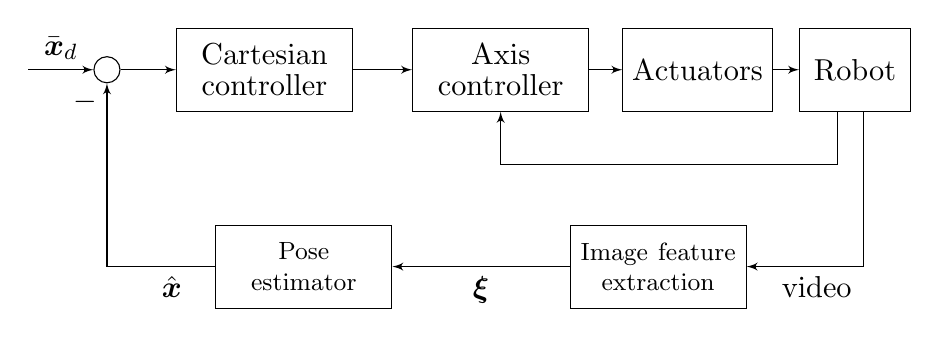
\begin{tikzpicture}
		\node [input] (input) {};
		\node [sum] at (1.,0.) (sum) {};
		\node [block, text width=2cm, align=center] (controller) at (3,0) {Cartesian controller};
		\node [block, text width=2cm, align=center] (axis-controller) at (6,0) {Axis controller};
		\node [block] (actuators) at (8.5,0) {Actuators};
		\node [block] (robot) at (10.5,0) {Robot};
		\node [block, text width=2cm, align=center] (image-processor) at (8,-2.5) {\small Image feature extraction};
		\node [block, text width=2cm, align=center] (computer-vision) at (3.5,-2.5) {\small Pose estimator};

		\draw [->] (input) -- node {$\bar{\vect{x}}_d$} (sum);
		\draw [->] (sum) -- (controller);
		\draw [->] (actuators) -- (robot);
		\draw [->] ([xshift=0.5cm]robot) |- node [pos=.7] {video} (image-processor);
		\draw [->] ([xshift=-0.5cm]robot) |- (8,-1.2) -| (axis-controller);
		\draw [->] (axis-controller) -- (actuators);
		\draw [->] (controller) -- (axis-controller);
		\draw [->] (computer-vision) -| node [pos=0.95] {$-$} node [pos=0.2] {$\hat{\vect{x}}$} (sum);
		\draw [->] (image-processor) -- node {$\vect{\xi}$} (computer-vision);
	\end{tikzpicture}
	\caption{Dynamic look and move position based}
	\label{fig:dynamic-look-move-position-based}
\end{figure}

\begin{figure}
	\centering
	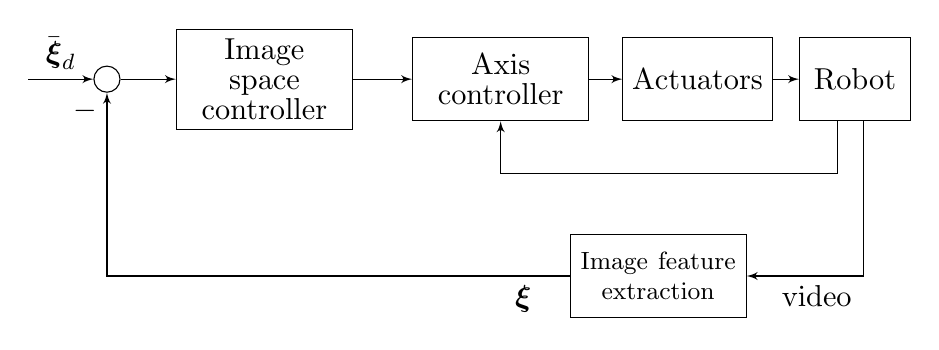
\begin{tikzpicture}
		\node [input] (input) {};
		\node [sum] at (1.,0.) (sum) {};
		\node [block, text width=2cm, align=center] (controller) at (3,0) {Image space controller};
		\node [block, text width=2cm, align=center] (axis-controller) at (6,0) {Axis controller};
		\node [block] (actuators) at (8.5,0) {Actuators};
		\node [block] (robot) at (10.5,0) {Robot};
		\node [block, text width=2cm, align=center] (image-processor) at (8,-2.5) {\small Image feature extraction};

		\draw [->] (input) -- node {$\bar{\vect{\xi}}_d$} (sum);
		\draw [->] (sum) -- (controller);
		\draw [->] (actuators) -- (robot);
		\draw [->] ([xshift=0.5cm]robot) |- node [pos=.7] {video} (image-processor);
		\draw [->] ([xshift=-0.5cm]robot) |- (8,-1.2) -| (axis-controller);
		\draw [->] (axis-controller) -- (actuators);
		\draw [->] (controller) -- (axis-controller);
		\draw [->] (image-processor) -| node [pos=0.95] {$-$} node [pos=0.05] {$\vect{\xi}$} (sum);
	\end{tikzpicture}
	\caption{Dynamic look and move image based}
	\label{fig:dynamic-look-move-image-based}
\end{figure}

\begin{figure}
	\centering
	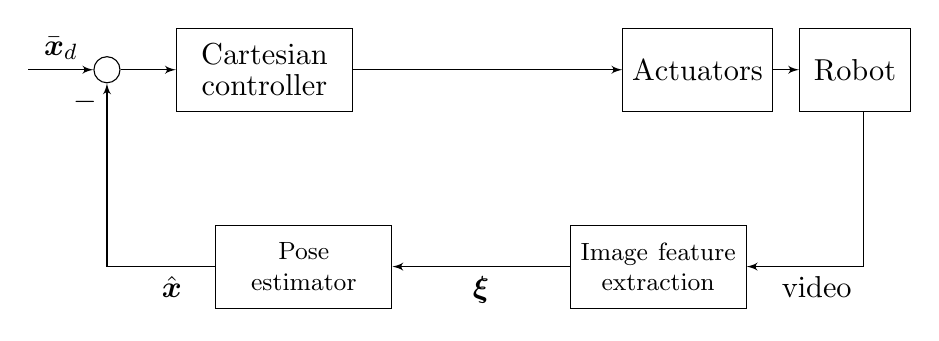
\begin{tikzpicture}
		\node [input] (input) {};
		\node [sum] at (1.,0.) (sum) {};
		\node [block, text width=2cm, align=center] (controller) at (3,0) {Cartesian controller};
		\node [block] (actuators) at (8.5,0) {Actuators};
		\node [block] (robot) at (10.5,0) {Robot};
		\node [block, text width=2cm, align=center] (image-processor) at (8,-2.5) {\small Image feature extraction};
		\node [block, text width=2cm, align=center] (computer-vision) at (3.5,-2.5) {\small Pose estimator};

		\draw [->] (input) -- node {$\bar{\vect{x}}_d$} (sum);
		\draw [->] (sum) -- (controller);
		\draw [->] (actuators) -- (robot);
		\draw [->] ([xshift=0.5cm]robot) |- node [pos=.7] {video} (image-processor);
		\draw [->] (controller) -- (actuators);
		\draw [->] (computer-vision) -| node [pos=0.95] {$-$} node [pos=0.2] {$\hat{\vect{x}}$} (sum);
		\draw [->] (image-processor) -- node {$\vect{\xi}$} (computer-vision);
	\end{tikzpicture}
	\caption{Visual servoing position based}
	\label{fig:visual-servoing-position-based}
\end{figure}

\begin{figure}
	\centering
	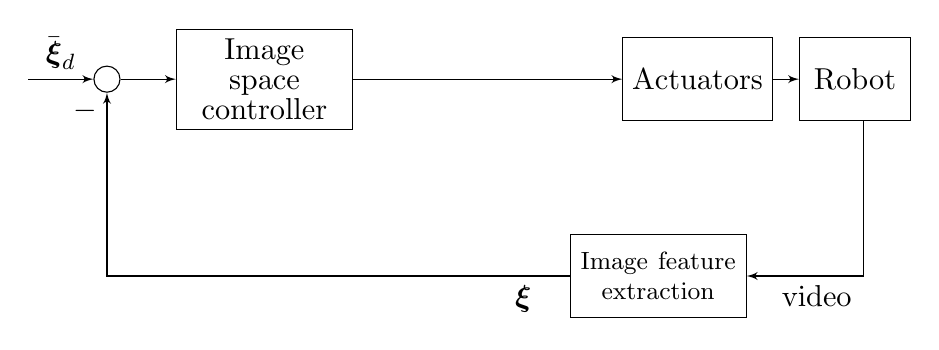
\begin{tikzpicture}
		\node [input] (input) {};
		\node [sum] at (1.,0.) (sum) {};
		\node [block, text width=2cm, align=center] (controller) at (3,0) {Image space controller};
		\node [block] (actuators) at (8.5,0) {Actuators};
		\node [block] (robot) at (10.5,0) {Robot};
		\node [block, text width=2cm, align=center] (image-processor) at (8,-2.5) {\small Image feature extraction};

		\draw [->] (input) -- node {$\bar{\vect{\xi}}_d$} (sum);
		\draw [->] (sum) -- (controller);
		\draw [->] (actuators) -- (robot);
		\draw [->] ([xshift=0.5cm]robot) |- node [pos=.7] {video} (image-processor);
		\draw [->] (controller) -- (actuators);
		\draw [->] (image-processor) -| node [pos=0.95] {$-$} node [pos=0.05] {$\vect{\xi}$} (sum);
	\end{tikzpicture}
	\caption{Visual servoing image based}
	\label{fig:visual-servoing-image-based}
\end{figure}

\subsection{Image based schema}

Design an image based control is a critical task;
we need to relate motion of the camera with motion of the features in the image.

Let us consider a fixed point $\vect{P}$ in the space and the camera frame $c$, we can state

\[ \vect{P}^w = \vect{O}_c^w(t) + \matr{R}_c^w(t) \vect{P}^c(t) \]

differentiating in time

\[ \vect{0} = \dot{\vect{O}}_c^w + \dot{\matr{R}}_c^w \vect{P}^c + \matr{R}_c^w \dot{\vect{P}}^c \]

and find the solution for $\dot{\vect{P}}^c$

\[ \dot{\vect{P}}^c = - \dot{\vect{O}}_c^c - \dot{\matr{R}}_c^c \vect{P}^c \]

remembering that $\dot{\matr{R}} \vect{P} = \vect{\omega} \times \vect{P}$ we get

\[ \dot{\vect{P}}^c = - \dot{\vect{O}}_c^c - \vect{\omega}_c^c \times \vect{P}^c \]

where all the vector are expressed in the camera frame.

Define

\[
	\vect{P}^c = \begin{bmatrix} X \\ Y \\ Z \end{bmatrix} \quad
	\vect{\omega}_c^c = \begin{bmatrix} \omega_x \\ \omega_y \\ \omega_z \end{bmatrix} \quad
	\dot{\vect{O}}_c^c = \begin{bmatrix} \dot{O}_x \\ \dot{O}_y \\ \dot{O}_z \end{bmatrix}
\]

we can write

\begin{gather*}
	\dot{X} = Y\omega_z - Z\omega_y - \dot{O}_x \\
	\dot{Y} = Z\omega_x - X\omega_z - \dot{O}_y \\
	\dot{Z} = X\omega_y - Y\omega_x - \dot{O}_z
\end{gather*}

remembering \autoref{eq:projected_point} we get

\begin{gather*}
	\dot{X} = \frac{x}{\lambda} Z\omega_z - Z\omega_y - \dot{O}_x \\
	\dot{Y} = Z\omega_x - \frac{y}{\lambda} Z\omega_z - \dot{O}_y \\
	\dot{Z} = \frac{x}{\lambda} Z\omega_y - \frac{y}{\lambda} Z\omega_x - \dot{O}_z
\end{gather*}

Differentiating in time projective coordinate from \autoref{eq:projected_point}

\begin{gather*}
	\dot{x} = \lambda \frac{d}{dt}\frac{X}{Z} = \lambda \frac{\dot{X}Z - X\dot{Z}}{Z^2} \\
	\dot{y} = \lambda \frac{d}{dt}\frac{Y}{Z} = \lambda \frac{\dot{Y}Z - Y\dot{Z}}{Z^2}
\end{gather*}

now we can finally write the relation between motion of the camera to the motion of the image's features

\[
	\begin{bmatrix} \dot{x} \\ \dot{y} \end{bmatrix} =
	\matr{L}(\lambda, x, y, Z)
	\begin{bmatrix} \dot{\vect{O}}_c^c \\ \vect{\omega}_c^c \end{bmatrix}
\]

where

\[
	\matr{L}(\lambda, x, y, Z) =
	\begin{bmatrix}
		-\frac{\lambda}{Z} & 0 & \frac{x}{Z} & \frac{xy}{\lambda} & -\frac{\lambda^2 + x^2}{\lambda}  & y \\
		0 & -\frac{\lambda}{Z} & \frac{y}{Z} & \frac{\lambda^2 + y^2}{\lambda} & -\frac{xy}{\lambda} & -x
	\end{bmatrix}
\]

and it is called \textbf{interaction matrix}.

\subsubsection{Interaction matrix}

The \textbf{interaction matrix} is a $2\times6$ matrix, it depends on variable values $x$, $y$ and $Z$.
If it decomposed

\[
	\begin{bmatrix} \dot{x} \\ \dot{y} \end{bmatrix} =
	\matr{L}_O(\lambda, x, y, Z) \dot{\vect{O}}_c^c + \matr{L}_\omega(\lambda, x, y) \vect{\omega}_c^c
\]

we can see that the rotation part does not depend on depth $Z$.

Due to the shape of it, we can state that exist an associated null space with dimension of 4, so there are four types of camera movement that not produce any change of the feature in the projective image.

\subsubsection{Image Jacobian}

If we try to bind camera speed we write

\[ \begin{bmatrix} \dot{\vect{O}}_c^c \\ \vect{\omega}_c^c \end{bmatrix} = \matr{T}_w^c(\q) \matr{J}(\q)\dq \]

where $ \matr{T}_w^c(\q)$ is the coordinate transformation between world and camera frame, and $\matr{J}(\q)$ is the robot \textbf{geometrical Jacobian}.
So, we can write

\[
	\begin{bmatrix} \dot{x} \\ \dot{y} \end{bmatrix} =
	\matr{L}(\lambda, x, y, Z) \matr{T}_w^c(\q) \matr{J}(\q)\dq = \matr{J}_I(\lambda, x, y, Z, \q) \dq
\]

where $\matr{J}_I$ is the \textbf{image Jacobian}.

The $Z$ parameter is clearly not available, but it can be estimated based on apriori information.

Now the \textbf{image Jacobian} can be used to design the control law in the image based scheme.

\[ \dq = \matr{J}_I^\psinv \left(\dot{\xi}_d + k (\xi_d - \xi)x\right) + \left(\matr{I} - \matr{J}_I^\psinv\matr{J}_I \right)\dq_0 \]
\include{chapters/8-collaborative-robotics}

\printindex

\end{document}